\chapter{数值实验与结果}

\section{数值实验与结果}
\label{sec:experiments}

本节给出若干数值算例，用于系统评估 DeepRTE 在辐射传输方程求解中的精度与效率。实际应用中，RTE~\eqref{eq:rte} 定义在三维空间变量 $\br\in\mathbb{R}^3$ 与角变量 $\bOmega\in\sS^2$ 上，对应 $d=3$，因此为六维问题。通过适当的变量变换与对称性分析，可以将其约化为低维模型，从而降低数值计算的整体复杂度。

在笛卡尔坐标系下，记
\begin{equation}
    \bOmega=(c,s,\zeta), \quad c =
        {\left(1-\zeta^{2}\right)}^{\frac{1}{2}} \cos\theta, \quad s =
        {\left(1-\zeta^{2}\right)}^{\frac{1}{2}} \sin\theta, \quad \text{for }|\zeta| \leq 1.
\end{equation}
令总截面 $\mut$ 与散射截面 $\mus$ 仅依赖于平面坐标 $(x,y)$，且强度 $I$ 在 $z$ 方向上均匀，则定义
\begin{equation}
    \tilde{I}(x, y,\zeta,\theta) = \frac{1}{2}\bigl[I(x,y,z,c,s,\zeta) + I(x,y,z,c,s,-\zeta)\bigr],
\end{equation}
以及
\begin{equation}
    \tilde{p}(\zeta,\theta,\zeta^*, \theta^*) = \frac{1}{2}\bigl[p(c,s,\zeta, c^*,s^*,\zeta^*) + p(c,s,\zeta, c^*,s^*,-\zeta^*)\bigr],
\end{equation}
则两者均与 $z$ 无关，且关于 $\zeta$ 为偶函数。由此，方程~\eqref{eq:rte-with-bc} 可约化为
\begin{equation}
    \bigl(c\partial_x \tilde{I}(x,y,\zeta,\theta)+s\partial_y
    \tilde{I}(x,y,\zeta,\theta)\bigr)+\mut \,\tilde{I}(x,y,\zeta,\theta)=\frac{\mus}{2\pi}\int_{0}^{1}
    \int_0^{2\pi} \tilde{p}(\zeta, \theta, \zeta^*,\theta^*) \,\tilde{I}(x,y,\zeta^*,\theta^*) \,\diff{\theta^*}\diff{\zeta^*},
\end{equation}
配以入射边界条件
\begin{equation}
    \tilde{I}(x,y,\bOmega)=\tilde{I}_{-}(x,y,\bOmega), \quad \text{当 }
    \bOmega\cdot\bm{n}<0,\quad (x, y)\in\partial D.
\end{equation}

相函数 $p$ 是辐射传输方程中的关键组成部分，通常仅依赖入射与出射方向之间的夹角。本文采用归一化的 Henyey--Greenstein（H-G）相函数作为各向异性散射的代表性模型：
\begin{equation}
    p(\bOmega,\bOmega^*) = p(\bOmega\cdot\bOmega^*) = \frac{1-g^2}{{\Bigl(1+g^2-2g\,(cc^*+ss^*+\zeta\zeta^*)\Bigr)}^{\frac{3}{2}}}.
\end{equation}
其中参数 $g$ 控制前向与后向散射的相对权重：$g=0$ 时对应各向同性散射，$g\to 1$ 时则对应高度前向集中的散射。虽然本文数值实验均基于 H-G 相函数，但算法本身可直接推广到其他散射模型。

\subsection{数据集构造}\label{sec:dataset-construction}

训练集与测试集均由传统数值方法生成，主要采用扫掠法（sweeping method）。
\todo[inline]{~\cite{koch1991solution,zeyao2004parallel}}
相应的 MATLAB 与 Python 实现已开源于 \href{https://github.com/mazhengcn/rte-dataset}{rte-dataset} 仓库，便于复现实验与进行进一步比较。

\paragraph{计算区域与离散}
数值实验在矩形空间区域 $D = [0, 1]\times[0, 1]\subset \mathbb{R}^2$ 以及角度空间 $\mathbb{S}^{2}$ 上进行。每个空间方向均采用 $40$ 个等间距网格点。

\paragraph{角度求积点}
角度求积点选取为区间 $[-1,1]$ 上 $2N$ 阶标准勒让德多项式的正根。本文取 $N=3$，对应的求积点与权重列于表~\ref{tab:quadrature}。

\begin{table}[!htp]
    \centering
    \begin{tabular}{ccccc}
        \toprule
        $\zeta_i$ & $\theta_i$ & $c_i$     & $s_i$     & $4 w_i$   \\
        \midrule
        0.2386192 & $\pi$/12   & 0.9380233 & 0.2513426 & 0.1559713 \\
        0.2386192 & 3$\pi$/12  & 0.6866807 & 0.6866807 & 0.1559713 \\
        0.2386192 & 5$\pi$/12  & 0.2513426 & 0.9380233 & 0.1559713 \\
        0.6612094 & $\pi$/8    & 0.6930957 & 0.2870896 & 0.1803808 \\
        0.6612094 & 3$\pi$/8   & 0.2870896 & 0.6930957 & 0.1803808 \\
        0.9324695 & $\pi$/4    & 0.2554414 & 0.2554414 & 0.1713245 \\
        \bottomrule
    \end{tabular}
    \bicaption{角度求积点及其权重。$\zeta_i$ 与 $\theta_i$ 为速度空间求积点，$c_i$ 与 $s_i$ 分别为对应的余弦与正弦值，$w_i$ 为求积权重。}{Angular quadrature points and weights of the quadrature set. $\zeta_i$ and $\theta_i$ are the quadrature points of the velocity space, $c_i$ and $s_i$ are the corresponding cosine and sine values, and $w_i$ is the quadrature weight.}\label{tab:quadrature}
\end{table}

\paragraph{截面系数}
总截面 $\mu_t(x,y)$ 与散射截面 $\mu_s(x,y)$ 在子区域 $D_\mu = [0.4, 0.6] \times [0.4, 0.6]$ 上随机取值，其余区域取常数，具体定义为
\begin{equation} \label{eq:coefficients_definition}
    \begin{aligned}
        \mu_t(x,y) & =
        \begin{cases}
            U_t, \quad \text{其中 } U_t \sim \mathcal{U}(5,7), & \text{若 } (x,y) \in D_\mu,    \\
            10,                                              & \text{若 } (x,y) \notin D_\mu,
        \end{cases} \\
        \mu_s(x,y) & =
        \begin{cases}
            U_s, \quad \text{其中 } U_s \sim \mathcal{U}(2,4), & \text{若 } (x,y) \in D_\mu,    \\
            5,                                               & \text{若 } (x,y) \notin D_\mu.
        \end{cases}
    \end{aligned}
\end{equation}

\paragraph{训练集边界条件}
训练数据集中采用 Delta 函数型入射边界条件，并用高斯函数进行近似。入射边界条件具体为
\begin{equation}\label{eq:bc-condition}
    \centering
    \left \{ % tex-fmt: skip
    \begin{aligned}
         & I_-(x=0,y,c>0,s;x_l^{\prime}=0,
        y_l^{\prime},c_l^{\prime},s_l^{\prime})
        =\delta_{\{y_l^{\prime}\}}^{\sigma_{\br}}(y)\delta^{\sigma_{\bOmega}}(c - c_l')\delta^{\sigma_{\bOmega}}(s - s_l'),
        \\
         & I_-(x=1,y,c<0,s;x_r^{\prime}=1,
        y_r^{\prime},c_r^{\prime},s_r^{\prime})
        =\delta_{\{y_r^{\prime}\}}^{\sigma_{\br}}(y)\delta^{\sigma_{\bOmega}}(c - c_r')\delta^{\sigma_{\bOmega}}(s - s_r'),
        \\
         & I_-(x,y=0,c,s>0;x_b^{\prime},y_b^{\prime}=0, c_b^{\prime},
        s_b^{\prime})
        =\delta_{\{x_b^{\prime}\}}^{\sigma_{\br}}(x)\delta^{\sigma_{\bOmega}}(c - c_b')\delta^{\sigma_{\bOmega}}(s - s_b'),
        \\
         & I_-(x,y=1,c,s<0;x_t^{\prime},y_t^{\prime}=1,c_t^{\prime},
        s_t^{\prime})
        =\delta_{\{x_t^{\prime}\}}^{\sigma_{\br}}(x)\delta^{\sigma_{\bOmega}}(c - c_t')\delta^{\sigma_{\bOmega}}(s - s_t'),
    \end{aligned}
    \right. % tex-fmt: skip
\end{equation}
其中，$y_l'$（left）、$y_r'$（right）、$x_b'$（bottom）与 $x_t'$（top）分别为对应边界上高斯束中心的坐标，从离散网格点中均匀随机选取。角变量 $c_l'$、$c_r'$、$c_b'$、$c_t'$ 及 $s_l'$、$s_r'$、$s_b'$、$s_t'$ 则从满足入射条件的离散速度方向中均匀采样。空间与角度方向上的尺度参数分别满足
\begin{equation}
    \sigma_{\br} \sim \mathcal{U}(0.005\sqrt{2},0.02\sqrt{2}), \quad \sigma_{\bOmega} \sim \mathcal{U}(0.005\sqrt{2},0.01\sqrt{2}).
\end{equation}

\paragraph{数据归一化}
在训练过程中，将强度 $I$ 归一化到区间 $[0, 1]$：
\begin{equation}
    I_{\text{norm}} = \frac{I - I_{\text{min}}}{I_{\text{max}} - I_{\text{min}}},
\end{equation}
其中 $I_{\text{min}}$ 与 $I_{\text{max}}$ 分别为数据集中观测到的最小与最大强度值。该归一化有助于稳定训练过程并提升收敛性能。

\paragraph{散射参数区间}
模型在三种不同散射强度区间上进行训练与测试，这些区间由散射不对称参数 $g\in[0,1]$ 划分：$g=0$ 表示各向同性散射，$g=1$ 表示极端前向散射。具体区间为
\begin{itemize}
    \item \textbf{近各向同性（Near isotropy）}: $ g \sim \mathcal{U}(0, 0.2)$，对应几乎各向同性散射，即粒子在各方向散射概率接近相同；
    \item \textbf{中度各向异性（Moderate anisotropy）}: $ g \sim \mathcal{U}(0.4, 0.6)$，对应中等强度的各向异性散射；
    \item \textbf{强前向散射（Highly forward peaking）}: $ g \sim \mathcal{U}(0.7, 0.9)$，对应粒子主要沿前向传播的强各向异性情形，此时粒子轨迹高度相关、位置与散射方向紧密耦合，边界条件的微小变化也可能显著影响解的行为。
\end{itemize}

上述数据集构造所用的超参数汇总于表~\ref{tab:dataset}。
\begin{table}[!htp]
    \centering
    \begin{tabular}{lp{0.3\textwidth}ll}
        \toprule
        类别                                         & 参数                                            & 符号                       & 取值/范围                                \\ \midrule
        \multirow{2}{*}{空间区域（Spatial domain）}      & 计算区域（Domain）                                  & $D$                      & ${[0,1]}^2$                          \\
                                                   & 子区域（Subdomain）                                & $D_\mu$                  & ${[0.4,0.6]}^2$                      \\
        \midrule
        \multirow{4}{*}{截面系数（Cross section）}       & \multirow{2}{*}{总截面（Total）}                   & \multirow{2}{*}{$\mut$}  & $D_\mu$ 内：$\mathcal{U}(5,7)$         \\
                                                   &                                               &                          & $D\backslash D_\mu$ 内：$10$           \\
                                                   & \multirow{2}{*}{散射截面（Scattering）}             & \multirow{2}{*}{$\mus$}  & $D_\mu$ 内：$\mathcal{U}(2,4)$         \\
                                                   &                                               &                          & $D\backslash D_\mu$ 内：$5$            \\
        \midrule
        \multirow{2}{*}{离散化（Discretization）}       & 空间网格点数（\# of mesh points）                     & $N_{\text{mesh}}$        & 40                                   \\
                                                   & 角度求积点数（\# of angular quadrature points）       & $N_\text{quad}$          & 24                                   \\ \midrule
        \multirow{5}{*}{边界条件（Boundary conditions）} & 光束空间中心坐标（Beam spatial centers）                & $y_l', y_r', x_b', x_t'$ & 从网格点中随机采样                            \\
                                                   & \multirow{2}{*}{光束角度求积点（Beam angular points）} & $c_l', c_r', c_b', c_t'$ & \multirow{2}{*}{从角度求积点中随机采样}         \\
                                                   &                                               & $s_l', s_r', s_b', s_t'$ &                                      \\
                                                   & 光束空间标准差（Beam spatial std dev）                 & $\sigma_{\br}$           & $\sqrt{2}\,\mathcal{U}(0.005, 0.02)$ \\
                                                   & 光束角度标准差（Beam angular std dev）                 & $\sigma_{\bOmega}$       & $\sqrt{2}\,\mathcal{U}(0.005, 0.01)$ \\
        \midrule
        \multirow{3}{*}{散射参数（Scattering）}          & \multirow{3}{*}{不对称参数（Asymmetry parameter）}   & \multirow{3}{*}{$g$}     & $\mathcal{U}(0,0.2)$                 \\
                                                   &                                               &                          & $\mathcal{U}(0.4,0.6)$               \\
                                                   &                                               &                          & $\mathcal{U}(0.7,0.9)$               \\
        \bottomrule
    \end{tabular}
    \bicaption{数据集构造中使用的超参数汇总。表中给出了计算区域、截面系数、离散参数、边界条件以及散射参数等设置。}{Summary of hyperparameters for dataset construction. This table details the computational domain, cross sections, discretization, boundary conditions, and other parameters used.}\label{tab:dataset}
\end{table}

\subsection{训练细节}

\paragraph{训练配置}

\begin{table}[!htp]
    \centering
    \begin{tabular}{ll}
        \toprule
        超参数（Hyperparameters）  & 取值（Value）                  \\ \midrule
        优化器（Optimizer）        & Adam                       \\
        学习率策略（Schedule）       & 余弦退火（Cosine annealing）     \\
        初始学习率                 & $1 \times 10^{-3}$         \\
        批大小（Batch size）       & 8                          \\
        训练轮数（Epochs）          & 5000                       \\
        训练样本数                 & 800                        \\
        验证样本数                 & 200                        \\
        配点数量（Collocation pts） & 128                        \\
        硬件（Hardware）          & 4$\times$ NVIDIA 4090 GPUs \\
        \bottomrule
    \end{tabular}
    \bicaption{模型训练超参数汇总。表中列出了优化器、学习率策略与初值、数据规模以及硬件配置等信息。}{Summary of model training hyperparameters. This table details the optimizer and training hyperparameters, including learning rate, dataset settings, and hardware information.}
    \label{tab:training_details}
\end{table}

模型训练采用 Adam 优化器与余弦退火（cosine annealing）学习率策略。对每个散射区间，各生成 $800$ 个训练样本与 $200$ 个验证样本。训练在四张 NVIDIA RTX 4090 GPU 上进行，共训练 $5000$ 个 epoch。初始学习率设为 $1 \times 10^{-3}$，batch size 取 $8$，损失函数中使用的 collocation 点数（见~\eqref{eq:collocation_points}）为 $128$。训练超参数如表~\ref{tab:training_details} 所示。

\paragraph{网络结构}
DeepRTE 的网络超参数列于表~\ref{tab:parameters}。网络由衰减模块与散射模块两部分构成，对应的层数、隐含维度、输出维度、多头注意力头数以及潜在特征维度等均在表中给出。

\begin{table}[!htp]
    \centering
    \begin{tabular}{lll}
        \toprule
        Module Name                  & Hyperparameters                          & Value \\ \midrule
        \multirow{7}{*}{Attenuation} & \texttt{num\_layer}
        $N_{\text{mlp}}$             & 4                                                \\
                                     & \texttt{hidden\_dim}  $d_{\text{mlp}}$   & $128$ \\
                                     & \texttt{output\_dim}  $d_{\text{model}}$ & $16$  \\
                                     & \texttt{num\_head}    $N_{\text{head}}$  & $2$   \\
                                     & \texttt{key\_dim}     $d_k$              & $32$  \\
                                     & \texttt{value\_dim}   $d_v$              & $32$  \\
                                     & \texttt{output\_dim}  $d_{\tau}$         & $2$   \\
        \midrule
        \multirow{2}{*}{Scattering}  & \texttt{num\_block}   $N_{\ell}$         & $2$   \\
                                     & \texttt{latent\_dim}  $d_{\text{model}}$ & $16$  \\
        \bottomrule
    \end{tabular}
    \bicaption{DeepRTE 网络超参数。网络由衰减模块与散射模块两部分构成，表中给出了层数、隐含维度、输出维度、多头数、键/值维度以及潜在特征维度等。}{DeepRTE network hyperparameters. The network consists of two modules: the attenuation module and the scattering module. The hyperparameters include the number of layers, hidden dimensions, output dimensions, number of heads, key dimensions, value dimensions, and latent dimensions.}\label{tab:parameters}
\end{table}

\subsection{结果分析}
\subsubsection{精度验证}
\label{sec:acc}

本小节评估 DeepRTE 的数值精度与计算效率。精度指标采用预测结果与真值之间的均方误差（MSE）以及均方根百分比误差（RMSPE）。所有结果均基于与训练集分布一致的验证数据集。

\begin{table}[!htp]
    \centering
    \begin{tabular}{@{}cccccc@{}}
        \toprule
        模型（Model）                & 参数量（\# of parameters）  & 散射区间（Scattering regime）       & $g$ 取值范围   & MSE ($\times 10^{-10}$) & RMSPE (\%) \\ \midrule
        \multirow{3}{*}{DeepRTE} & \multirow{3}{*}{37954} & 近各向同性（Near isotropy）          & (0, 0.2)   & 5.630                   & 2.827      \\ \cmidrule(l){3-6}
                                 &                        & 中度各向异性（Moderate anisotropy）   & (0.4, 0.6) & 5.453                   & 2.759      \\ \cmidrule(l){3-6}
                                 &                        & 强前向散射（Highly forward peaking） & (0.7, 0.9) & 7.223                   & 3.181      \\ \bottomrule
    \end{tabular}
    \bicaption{DeepRTE 在三种散射区间上的精度指标。所有验证样本与训练集分布一致，表中给出了各区间上的 MSE 与 RMSPE，均表现出较高精度。}{Accuracy validation of DeepRTE model across three distinct scattering regimes. All validation experiments were conducted on a dataset sharing the same distribution as the training dataset. The table demonstrates that the model achieves high accuracy with RMSPE consistently below 3.2\% across all regimes.}\label{tab:accuracy}
\end{table}

从表~\ref{tab:accuracy} 可见，在所有散射区间内，DeepRTE 的 MSE 均不超过 $7.3 \times 10^{-10}$，RMSPE 控制在 $3.2\%$ 以内，表明模型在不同散射强度下均具有较高精度。具体而言，在近各向同性区间中，MSE 为 $5.630 \times 10^{-10}$，RMSPE 为 $2.827\%$，在几乎各向同性情形下表现优异；在中度各向异性区间中，MSE 略有降低（$5.453 \times 10^{-10}$），RMSPE 为 $2.759\%$，精度相当；在强前向散射区间中，由于散射高度各向异性，问题更具挑战性，但模型仍能保持 $7.223 \times 10^{-10}$ 的 MSE 与 $3.181\%$ 的 RMSPE，反映出良好的鲁棒性。

表~\ref{tab:accuracy-figs} 给出了三个散射区间中代表性算例的可视化对比结果。对每个区间，我们依次展示：密度 $\Phi$ 的三维真值、二维投影真值、模型预测以及二者之差的绝对误差。

表~\ref{tab:time_compare} 给出了 DeepRTE 与传统方法在运行时间上的对比，用以体现本方法在效率方面的优势。快速扫掠法分别采用 CPU 与 GPU 两种实现：CPU 版本基于 Python（NumPy 与 SciPy），在 Intel(R) Xeon(R) Silver 4410Y（12 核）上运行，耗时约 $193.0$ 秒；GPU 版本基于 JAX，在多个设备之间进行数据分片、采用多 GPU 并行与 \texttt{jax.jit} JIT 编译（见算法~\ref{alg:fast-sweeping-gpu}），在 $4\times$ NVIDIA GeForce RTX 4090 上耗时约 $16.7$ 秒，相比 CPU 提升约 $11.6$ 倍。相比之下，DeepRTE 在相同的 $4\times$ RTX 4090 上完成一次推理仅需 $2.3$ 秒，相比 GPU 快速扫掠法进一步加速约 $7.3$ 倍，相比 CPU 基线则加速约 $83.9$ 倍，推理效率优势十分显著。

这些结果表明，DeepRTE 在不同散射参数设置下均能够较好地捕捉散射物理过程，在复杂的前向散射场景中仍能保持较低误差；同时，模型参数量仅约 $3.8\times 10^4$，推理效率较高，适合大规模高效模拟场景。

\begin{table}[!htp]
    \centering
    \begin{tabular}{@{}lccc@{}}
        \toprule
        方法（Method）   & 设备（Device）                    & 计算单元数量（Count） & 时间 Time (s) \\ \midrule
        快速扫掠法（CPU）   & Intel(R) Xeon(R) Silver 4410Y & 12 核（cores）   & 193.0       \\
        快速扫掠法（GPU）   & NVIDIA GeForce RTX 4090       & 4 GPUs        & 16.7        \\
        \midrule
        DeepRTE（GPU） & NVIDIA GeForce RTX 4090       & 4 GPUs        & 2.3         \\ \bottomrule
    \end{tabular}
    \bicaption{不同方法在 CPU 与 GPU 上的运行时间对比。快速扫掠法在 CPU 与 GPU 上分别耗时 193.0 s 与 16.7 s，而 DeepRTE 在 $4\times$ RTX 4090 上仅需 2.3 s，显著提升了推理效率。}{Runtime comparison. The conventional fast sweeping method requires 193.0 s on an Intel(R) Xeon(R) Silver 4410Y (12 cores) and 16.7 s on $4\times$ NVIDIA GeForce RTX 4090 GPUs ($11.6\times$ over CPU). By contrast, DeepRTE completes inference in 2.3 s on $4\times$ RTX 4090, achieving a $7.3\times$ speedup over the GPU fast sweeping method and an $83.9\times$ speedup relative to the CPU baseline.}
    \label{tab:time_compare}
\end{table}

\begin{algorithm}[!htp]
    \caption{多 GPU 快速扫掠法（Multi-GPU Fast-Sweeping Method）}\label{alg:fast-sweeping-gpu}
    \SetAlgoLined
    \KwIn{$\mut, \mus, \{c_k\}, \{s_k\}, \{w_{k'}\}, p, \Delta x, \Delta y, D, \text{tol}, \text{max\_iter}$}
    \KwOut{$I$}

    \BlankLine

    \emph{在 $D$ 个设备之间划分角通量与散射核}
    $M \gets n_v / D$\;

    \For{$d = 1,\dots,D$}{%
    \emph{在第 $d$ 个设备上初始化角通量与散射核，并复制截面系数}\
    $I^{d,[\ell]}_{i,j,k} \gets 0,\quad I^{d,[\ell]}_{i,j,k} \in \mathbb{R}^{n_x \times n_y \times M}$\;
    $p^d_{k,k'} \gets p_{k,k'},\quad k \in [(d-1)M, dM),\; k' \in [0,n_v)$\;
    $\mu_t^d,\mu_s^d \gets \mu_t,\mu_s$\;
    }

    \BlankLine

    \For{$\ell = 0,1,\dots,\text{max\_iter}-1$}{%
    \emph{步骤 1：跨设备收集角通量（全收集通信）}\
    $I^{[\ell]}_{i,j,k'} \gets \text{All-Gather}(\{I^{d,[\ell]}_{i,j,k}\}_{d=1}^D),\quad k' \in [0,n_v)$\;

    \emph{步骤 2：在各设备上计算局部散射矩（本地计算，无通信）}\
    \For{$d = 1,\dots,D$}{%
    $S^{d,[\ell]}_{i,j,k} \gets \displaystyle\sum_{k'=0}^{n_v-1} w_{k'}\,p^d_{k,k'}\,I^{[\ell]}_{i,j,k'},\quad k \in [(d-1)M, dM)$\;
    }

    \emph{步骤 3：在各设备上执行角度扫掠（本地计算，无通信）}\
    \For{$d = 1,\dots,D$}{%
    \For{$(i,j)$ \text{ in sweep order}}{%
    $I^{d,[\ell+1]}_{i,j,k} \gets \dfrac{c_k\dfrac{I^{d,[\ell]}_{i-1,j,k}}{\Delta x} + s_k\dfrac{I^{d,[\ell]}_{i,j-1,k}}{\Delta y} + (\mu_s)_{i,j}\,S^{d,[\ell]}_{i,j,k}}{\dfrac{c_k}{\Delta x} + \dfrac{s_k}{\Delta y} + (\mu_t)_{i,j}},\quad k \in [(d-1)M, dM)$\;
    }
    }

    \emph{步骤 4：检查收敛性}\
    \If{$\text{RelativeError}(I^{[\ell+1]}, I^{[\ell]}) < \text{tol}$}{%
        extbf{break}\;
    }
    }

    \BlankLine

    \emph{在所有设备之间收集最终角通量}\
    $I^{[\ell]} \gets \text{All-Gather}(\{I^{d,[\ell]}\}_{d=1}^D)$\;

    \Return{$I^{[\ell]}$}\;
\end{algorithm}

\begin{table}[!htp]
    \centering
    \begin{tabular}{>{\centering\arraybackslash}m{0.9cm}cccc}
        \toprule
        $g$                         & $\Phi_{\text{label}}$                                             & $\Phi_{\text{label}}$                                          & $\Phi_{\text{predict}}$                                      & $|\Phi_{\text{label}}- \Phi_{\text{predict}}|$                 \\
        \midrule
        \raisebox{5em}{$(0,0.2)$}   & 
\includegraphics[width=0.22\textwidth]{val_g0.1_phi_label_3d.pdf} & 
\includegraphics[width=0.20\textwidth]{val_g0.1_phi_label.pdf} & 
\includegraphics[width=0.20\textwidth]{val_g0.1_phi_pre.pdf} & 
\includegraphics[width=0.20\textwidth]{val_g0.1_phi_error.pdf} \\
        \raisebox{5em}{$(0.4,0.6)$} & 
\includegraphics[width=0.22\textwidth]{val_g0.5_phi_label_3d.pdf} & 
\includegraphics[width=0.20\textwidth]{val_g0.5_phi_label.pdf} & 
\includegraphics[width=0.20\textwidth]{val_g0.5_phi_pre.pdf} & 
\includegraphics[width=0.20\textwidth]{val_g0.5_phi_error.pdf} \\
        \raisebox{5em}{$(0.7,0.9)$} & 
\includegraphics[width=0.22\textwidth]{val_g0.8_phi_label_3d.pdf} & 
\includegraphics[width=0.20\textwidth]{val_g0.8_phi_label.pdf} & 
\includegraphics[width=0.20\textwidth]{val_g0.8_phi_pre.pdf} & 
\includegraphics[width=0.20\textwidth]{val_g0.8_phi_error.pdf} \\
        \bottomrule
    \end{tabular}
    \bicaption{不同散射区间下密度 $\Phi$ 预测结果的可视化比较：包括三维与二维真值、模型预测以及绝对误差图。}{Visual comparison of density $\Phi$ predictions across scattering regimes: ground truth (3D and 2D views), model predictions, and absolute errors for representative validation cases.}\label{tab:accuracy-figs}
\end{table}

\begin{figure}[!htp]
    \centering
    
\includegraphics[width=\textwidth]{train_loss.pdf}
    \bicaption{在 Delta 函数训练数据集上训练所得的损失曲线，展示了随 epoch 推进的收敛行为。}{Loss curve. Obtained from training the model on a delta function training dataset, illustrating the convergence behavior over epochs.}\label{fig:loss}
\end{figure}

\subsubsection{线性性质验证}\label{sec:linearity_val}

DeepRTE 的网络结构在设计时就有意保持了对入射边界函数 $I_{-}$ 的线性性质。根据~\eqref{eq:greens-integral-nn}，DeepRTE 中使用的神经网络 $G^{\text{NN}}$ 以积分形式表征了解算子 $\ANN$ 的核（即格林函数），因此在连续和离散层面上，DeepRTE 从 $I_{-}$ 到解的整体映射应当保持线性。

为验证这一结论，本节通过数值实验证明模型同时满足可加性与齐次性两条基本线性性质。所有实验均在固定的截面系数 $\mu_t,\mu_s$ 与相函数 $p$ 条件下进行，其具体设置为
\begin{equation}
    \mu_t(x,y) =
    \begin{cases}
        6,  & \text{若 } (x,y) \in D_\mu,    \\
        10, & \text{若 } (x,y) \notin D_\mu,
    \end{cases}
    \quad
    \mu_s(x,y) =
    \begin{cases}
        3, & \text{若 } (x,y) \in D_\mu,    \\
        5, & \text{若 } (x,y) \notin D_\mu,
    \end{cases}
    \quad
    g=0.5, \quad D_\mu = [0.4, 0.6]^2.
\end{equation}
下文中，记 DeepRTE 解算子为 $\ANN$（省略参数依赖）。

\paragraph{1. 可加性检验}
线性可加性要求：对应于两个入射边界之和的预测解，应等于分别求解后二者解的和，即
\begin{equation}\label{eq:additivity-val}
    \ANN(I_{-}^{(1)} + I_{-}^{(2)}) = \ANN I_{-}^{(1)} + \ANN I_{-}^{(2)}.
\end{equation}
我们首先选取验证集中的两个独立入射边界条件 $I_{-}^{(1)}$ 与 $I_{-}^{(2)}$，其形式均为~\eqref{eq:bc-condition}，并取
\begin{equation}
    I_{-}^{(1)}:
    \begin{cases}
        y_l'=0.3875,\; y_r'=0.6125,\; x_b'=0.6125,\; x_t'=0.3875,   \\
        c_l'=0.6931,\; c_r'=-0.6931,\; c_b'=0.2871,\; c_t'=-0.2871, \\
        s_l'=-0.2871,\; s_r'=0.2871,\; s_b'=0.6931,\; s_t'=-0.6931,
    \end{cases}
\end{equation}
以及
\begin{equation}
    I_{-}^{(2)}:
    \begin{cases}
        y_l'=0.1375,\; y_r'=0.8625,\; x_b'=0.8625,\; x_t'=0.1375,   \\
        c_l'=0.2871,\; c_r'=-0.2871,\; c_b'=-0.6931,\; c_t'=0.6931, \\
        s_l'=0.6931,\; s_r'=-0.6931,\; s_b'=0.2871,\; s_t'=-0.2871.
    \end{cases}
\end{equation}
此处方差取 $\sigma_{\br}=0.01$、$\sigma_{\bOmega}=0.0075$。我们计算~\eqref{eq:additivity-val} 左右两侧的 MSE：
\begin{equation}
    \ell(\ANN (I_{-}^{(1)}{+}I_{-}^{(2)}),\ANN I_{-}^{(1)} + \ANN I_{-}^{(2)})=1.581\times 10^{-19},
\end{equation}
可见二者几乎完全重合，从而验证了 DeepRTE 的可加性。

进一步地，我们比较合成边界 $I_{-}^{(1)}{+}I_{-}^{(2)}$ 下 DeepRTE 预测解 $\ANN (I_{-}^{(1)}{+}I_{-}^{(2)})$ 与数值求解器所得真解 $\mathcal{A}(I_{-}^{(1)}{+}I_{-}^{(2)})$ 之间的误差：MSE 为 $1.358\times10^{-8}$，RMSPE 为 $2.83\%$，说明模型在合成边界条件下仍能保持较高精度。相应的密度 $\Phi$ 可视化结果见图~\ref{fig:additivity}。

为了更一般地验证可加性，我们还在 100 个验证样本上进行统计实验。对每个样本的边界条件 $I_{-}^{(1)}$，随机选取另一样本边界 $I_{-}^{(2)}$，构造合成边界 $I_{-}^{(1)}{+}I_{-}^{(2)}$，并比较~\eqref{eq:additivity-val} 两侧。此时 MSE 与 RMSPE 分别为 $1.421\times 10^{-19}$ 与 $9.20\times10^{-6}\%$（见表~\ref{tab:linearity}），进一步印证了可加性。

\begin{figure}[!htp]
    \centering
    \begin{subfigure}[b]{0.30\textwidth}
        \centering
        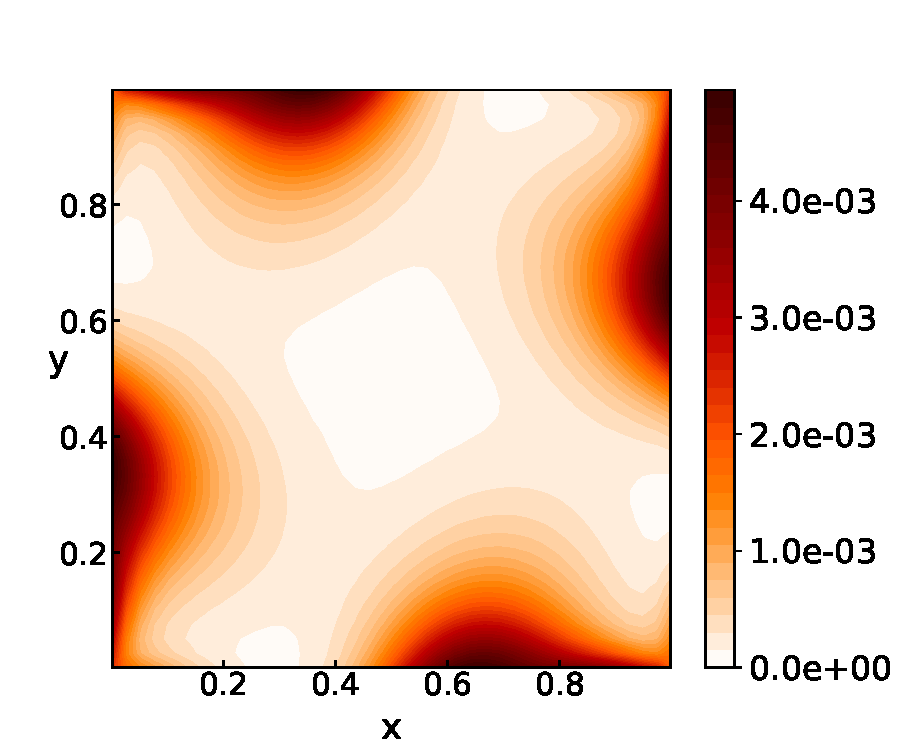
\includegraphics[width=\textwidth]{figures/delta_sigma_a3-sigma_t6-g0_5-r5-v9-phi_label.pdf}
        \caption{$\ANN (I_{-}^{(1)} + I_{-}^{(2)})$ 对应的密度 $\Phi$}
    \end{subfigure}
    \hfill
    \begin{subfigure}[b]{0.30\textwidth}
        \centering
        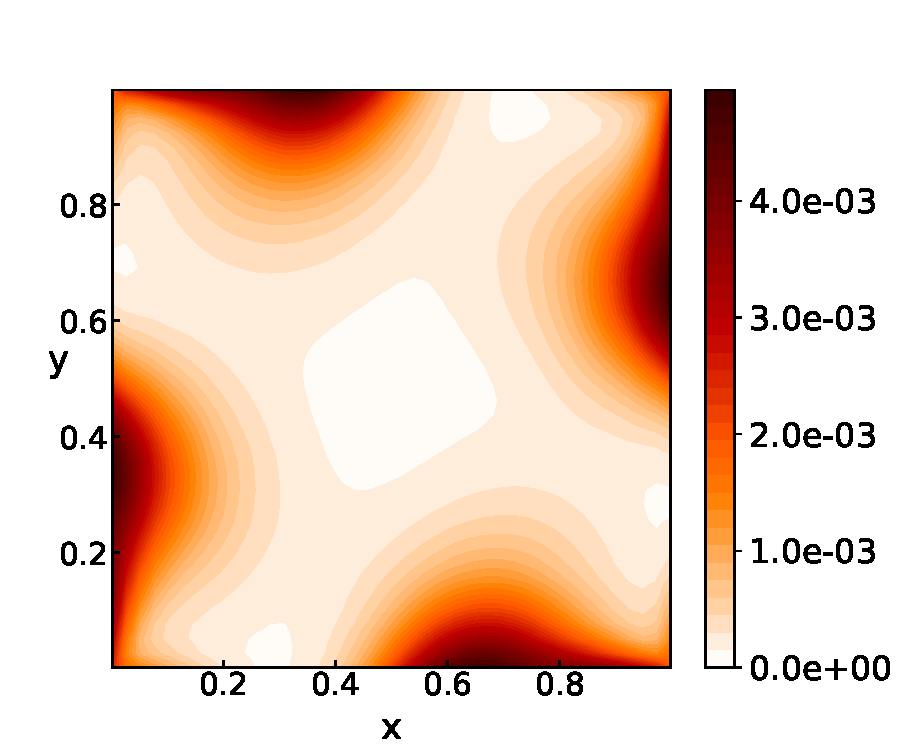
\includegraphics[width=\textwidth]{figures/delta_sigma_a3-sigma_t6-g0_5-r5-v9-phi_pre.pdf}
        \caption{$\ANN I_{-}^{(1)} + \ANN I_{-}^{(2)}$ 对应的密度 $\Phi$}
    \end{subfigure}
    \hfill
    \begin{subfigure}[b]{0.30\textwidth}
        \centering
        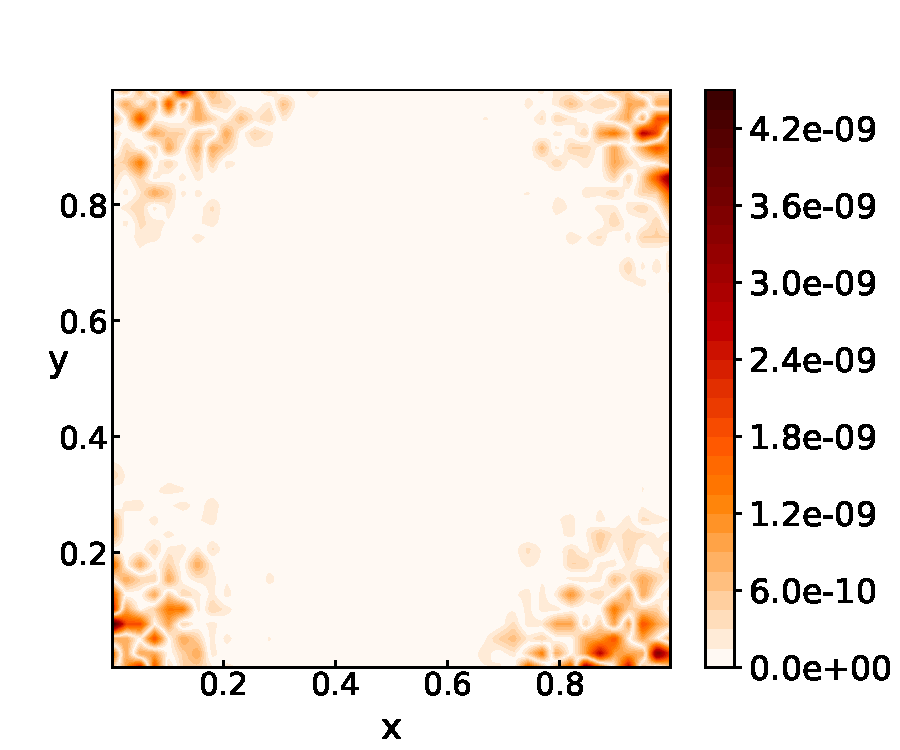
\includegraphics[width=\textwidth]{figures/delta_sigma_a3-sigma_t6-g0_5-r5-v9-phi_error.pdf}
        \caption{绝对误差}
    \end{subfigure}
    \bicaption{DeepRTE 可加性检验算例，参数取 $g=0.5$、$\mus=3$、$\mut=6$。}{Additivity verification of DeepRTE with $g=0.5$, $\mus=3$ and $\mut=6$.}
    \label{fig:additivity}
\end{figure}

\paragraph{2. 齐次性检验}
线性齐次性要求：若将入射边界整体按系数 $\alpha$ 放缩，则预测解也按同一系数放缩：
\begin{equation}\label{eq:homogeneity-val}
    \ANN(\alpha I_{-}) = \alpha \,\ANN I_{-}, \quad \forall\, \alpha \in \mathbb{R}.
\end{equation}
我们同样从验证集中选取边界条件 $I_{-}$：
\begin{equation}
    I_{-}:
    \begin{cases}
        y_l'=0.3875,\; y_r'=0.6125,\; x_b'=0.6125,\; x_t'=0.3875,   \\
        c_l'=0.6931,\; c_r'=-0.6931,\; c_b'=0.2871,\; c_t'=-0.2871, \\
        s_l'=-0.2871,\; s_r'=0.2871,\; s_b'=0.6931,\; s_t'=-0.6931,
    \end{cases}
\end{equation}
方差取 $\sigma_{\br}=0.01$、$\sigma_{\bOmega}=0.0075$，并令
\begin{equation}
    \alpha = 5.
\end{equation}
计算~\eqref{eq:homogeneity-val} 左右两侧的 MSE：
\begin{equation}
    \ell(\ANN (\alpha I_{-}), \alpha \,\ANN I_{-}) = 5.179\times 10^{-13},
\end{equation}
同样表明 DeepRTE 在数值上严格满足齐次性性质。

在此基础上，对于放缩边界 $\alpha I_{-}$，我们比较 DeepRTE 预测解 $\ANN (\alpha I_{-})$ 与数值求解器给出的真解 $\mathcal{A}(\alpha I_{-})$：MSE 为 $5.842\times10^{-9}$，RMSPE 为 $2.19\%$，说明在幅值放大的情形下模型依然保持较高精度。对应密度 $\Phi$ 的可视化结果如图~\ref{fig:homogeneity} 所示。

\begin{figure}[!htp]
    \centering
    \begin{subfigure}[b]{0.30\textwidth}
        \centering
        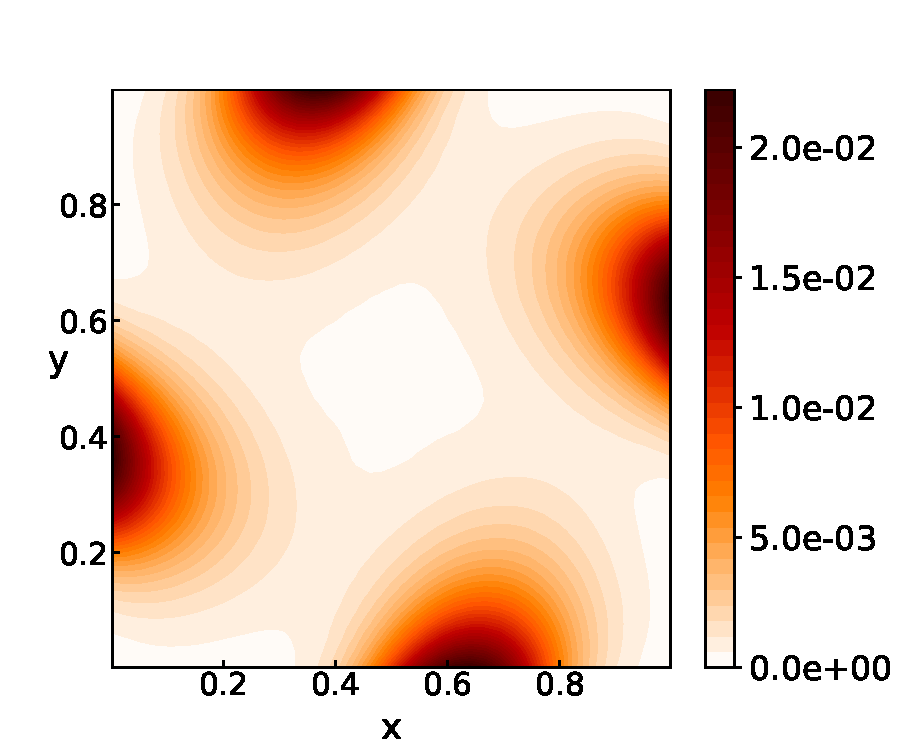
\includegraphics[width=\textwidth]{figures/delta-sigma_a3_sigma_t6-g0_5-r15-v3-phi_label.pdf}
        \caption{$\ANN (\alpha I_{-})$ 对应的密度 $\Phi$}
    \end{subfigure}
    \hfill
    \begin{subfigure}[b]{0.30\textwidth}
        \centering
        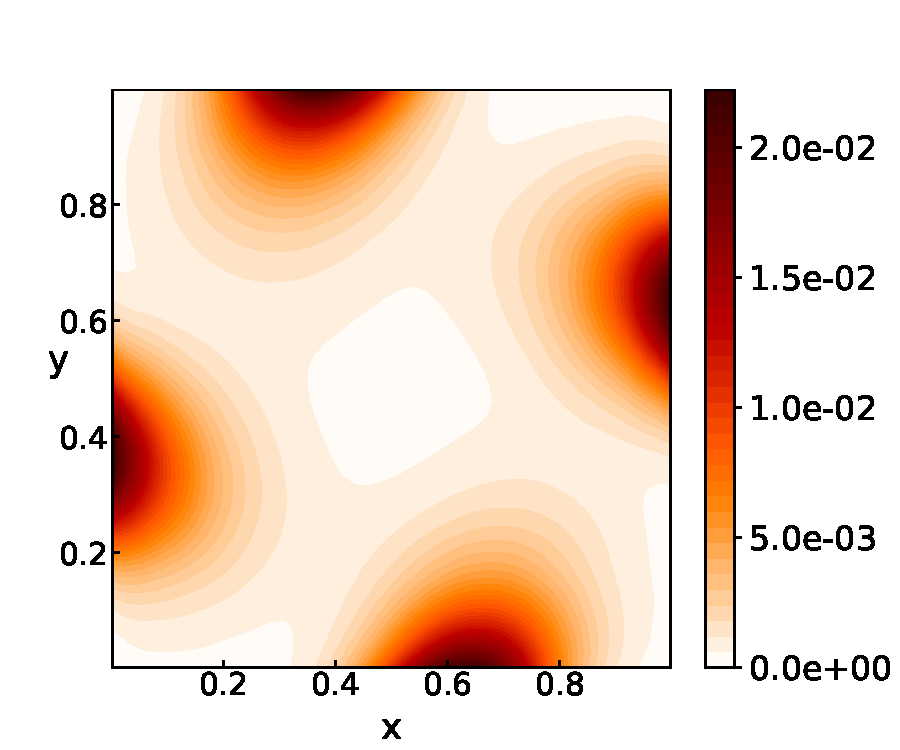
\includegraphics[width=\textwidth]{figures/delta-sigma_a3_sigma_t6-g0_5-r15-v3-phi_pre.pdf}
        \caption{$\alpha \,\ANN I_{-}$ 对应的密度 $\Phi$}
    \end{subfigure}
    \hfill
    \begin{subfigure}[b]{0.30\textwidth}
        \centering
        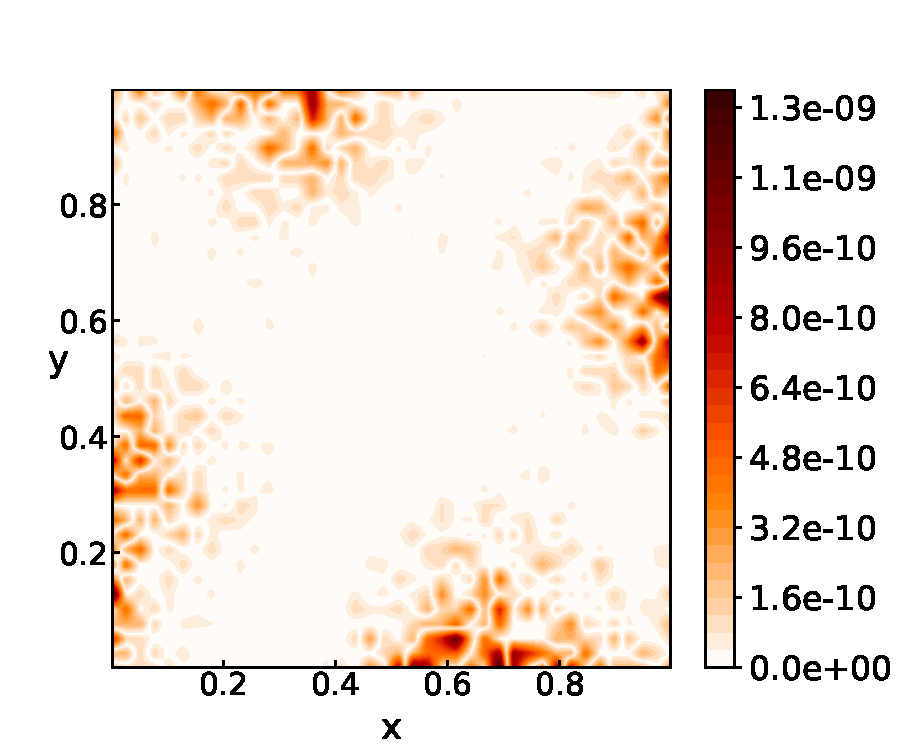
\includegraphics[width=\textwidth]{figures/delta-sigma_a3_sigma_t6-g0_5-r15-v3-phi_error.pdf}
        \caption{绝对误差}
    \end{subfigure}
    \bicaption{DeepRTE 齐次性检验算例，参数取 $g=0.5$、$\mus=3$、$\mut=6$、$\alpha=5$。}{Homogeneity verification with $g=0.5$, $\mus=3$, $\mut=6$ and $\alpha=5$.}\label{fig:homogeneity}
\end{figure}

同样地，我们在 100 个验证样本上统计检验齐次性。令缩放因子 $\alpha \sim \mathcal{U}(0,5)$，对每个原始边界条件 $I_{-}$ 构造 $\alpha I_{-}$，比较~\eqref{eq:homogeneity-val} 两侧。此时 MSE 与 RMSPE 分别为 $2.804\times 10^{-13}$ 与 $1.01\times 10^{-5}\%$，结果见表~\ref{tab:linearity}。

\begin{table}[!htp]
    \centering
    \begin{tabular}{lcc}
        \toprule
                         & MSE                    & RMSPE($\%$)          \\
        \midrule
        可加性（Additivity）  & $1.421\times 10^{-19}$ & $9.20\times 10^{-6}$ \\
        齐次性（Homogeneity） & $2.804\times 10^{-13}$ & $1.01\times 10^{-5}$ \\
        \bottomrule
    \end{tabular}
    \bicaption{在 $g=0.5$、与训练集分布一致的验证数据上对可加性与齐次性进行统计检验的结果。}{Additivity and homogeneity verification on 100 validation samples with the same distribution as the training dataset at $g=0.5$ (see Sec.~\ref{sec:acc}).}\label{tab:linearity}
\end{table}

\paragraph{3. 线性组合与误差分解}
前述可加性与齐次性表明：对于任意入射边界 $I_{-}$，DeepRTE 的泛化误差可以如定理~\ref{thm:error-estimate} 所示进行分解。本小节通过一个平滑入射边界算例，对该误差分解进行经验验证，并评估各个误差分量的相对量级。

考虑只在左边界施加平滑入射、其余边界为零的情形：
\begin{equation}
    \left \{ % tex-fmt: skip
    \begin{aligned}
         & I_-(x=0,y,c>0,s) = \sin(\pi y), \\
         & I_-(x=1,y,c<0,s) = 0,           \\
         & I_-(x,y=0,c,s>0) = 0,           \\
         & I_-(x,y=1,c,s<0) = 0.
    \end{aligned}
    \right. % tex-fmt: skip
\end{equation}

按照~\eqref{eq:particle-approx} 与~\eqref{eq:delta_defination}，仅需对左边界进行粒子近似：
\begin{equation}
    I_-(x=0,y,c>0,s) = \sin(\pi y) \approx \sum_{i=0}^{39} w_{i} \,\delta^{\sigma_{\br}}_{\{y_i\}}(y),
\end{equation}
其中 $\{y_i\}$ 为均匀网格中心，$g=0.5$、$\sigma_{\br} = 0.01$，并根据~\cite{chertock2017practical} 第 2.1 节取
\begin{equation}
    w_i=\frac{1}{40}\sin(\pi y_i).
\end{equation}

以数值解为参考解 $I^{\text{ref}}$，我们依次计算以下误差（所有 $L^2$ 误差均采用离散网格上的求积近似）：首先是正则化 Delta 近似误差
\begin{equation}
    \|I_{-} - I^{40}_{-,0.01}\|_{L^2} \approx \frac{1}{160}\bigl\|I_{(x=0,y,c>0,s)} - \sum_{i=0}^{39} w_{i} \,\delta^{\sigma_{\br}}_{\{y_i\}}(y)\bigr\|_{\ell^2}=4.799\times 10^{-5},
\end{equation}
以及
\begin{equation}
    \|\ANN_{\theta^*}(I_{-} - I^{40}_{-,0.01})\|_{L^2}\approx 2.190\times 10^{-7}, \quad
    \|\mathcal{A}(I_{-} - I^{40}_{-,0.01})\|_{L^2} \approx 2.208\times 10^{-7},
\end{equation}
最后是关于粒子近似的泛化误差项
\begin{equation}
    \| (\ANN_{\theta^*} - \mathcal{A}) I^{40}_{-,0.01}\|_{L^2}
    =\Bigl\|\sum_{i=0}^{39}w_i(\ANN_{\theta^*} - \mathcal{A}) \,\delta^{\sigma_{\br}}_{\{y_i\}}(y)\Bigr\|_{L^2} \leq \sum_{i=0}^{39}|w_i|\,\|(\ANN_{\theta^*} - \mathcal{A}) \,\delta^{\sigma_{\br}}_{\{y_i\}}(y)\|_{L^2} \approx 8.385\times 10^{-5}.
\end{equation}
由此得到总误差上界约为 $8.385\times 10^{-5}$。直接计算原边界条件下的推理误差
\begin{equation}
    \|(\ANN_{\theta^*} - \mathcal{A}) I_{-}\|_{L^2} \approx 1.888\times 10^{-5},
\end{equation}
明显低于上述理论上界，从数值上支持了定理~\ref{thm:error-estimate} 的误差分解结论。

\subsubsection{迁移学习与零样本性能}

本小节考察 DeepRTE 框架在迁移学习与零样本（Zero-Shot）场景下的表现。迁移学习允许模型将某一任务上学到的知识迁移到相关任务，以提升后者的性能；零样本能力则指在不额外训练的情况下，将模型直接应用于全新的条件。为展示 DeepRTE 在 RTE 问题上的此类能力——特别是其在几乎不做额外训练的前提下，适应新边界条件的能力——我们首先在 Delta 函数型入射边界条件数据集上训练模型，以学习 RTE 的基本物理规律；随后，在与训练集分布完全不同的边界条件上对模型进行测试，评估其泛化与零样本外推性能。

具体而言，我们考虑以下三类典型边界条件：
\begin{itemize}
    \item \textbf{Case I（常值边界条件）}: 从 Delta 函数边界条件外推到常值源项，用于评估模型的基础泛化能力；
    \item \textbf{Case II（三角函数边界条件）}: 通过正弦函数在空间方向上引入变化，用于检验模型处理平滑、周期且空间相关边界条件的能力；
    \item \textbf{Case III（速度相关边界条件）}: 在空间与速度方向上同时引入非线性依赖，用于评估模型对复杂、方向相关边界条件的适应能力。
\end{itemize}

\paragraph{Case I. 常值边界条件}
该算例的入射边界条件为
\begin{equation}
    \left \{
    \begin{aligned}
         & I_-(x=0,y,c>0,s) =1,  \\
         & I_-(x=1,y,c<0,s) = 0, \\
         & I_-(x,y=0,c,s>0) =0,  \\
         & I_-(x,y=1,c,s<0) =0,
    \end{aligned}
    \right.
\end{equation}

\begin{figure}[!htp]
    \centering
    \begin{subfigure}[b]{0.24\textwidth}
        \centering
        
\includegraphics[width=\textwidth]{test_bc1_g0.1_label_3d.pdf}
        \caption{$\Phi_{\text{label}}$ (3D)}\label{fig:caseI_label_3d}
    \end{subfigure}
    \hfill
    \begin{subfigure}[b]{0.24\textwidth}
        \centering
        
\includegraphics[width=\textwidth]{test_bc1_g0.1_label.pdf}
        \caption{$\Phi_{\text{label}}$}\label{fig:caseI_label}
    \end{subfigure}
    \hfill
    \begin{subfigure}[b]{0.24\textwidth}
        \centering
        
\includegraphics[width=\textwidth]{test_bc1_g0.1_pre.pdf}
        \caption{$\Phi_{\text{predict}}$}\label{fig:caseI_predict}
    \end{subfigure}
    \hfill
    \begin{subfigure}[b]{0.24\textwidth}
        \centering
        
\includegraphics[width=\textwidth]{test_bc1_g0.1_error.pdf}
        \caption{Absolute error}\label{fig:caseI_error}
    \end{subfigure}
    \bicaption{常值边界条件（Case I）下的评估结果，散射核参数 $g\in (0,0.2)$。预测解的 RMSPE 为 2.573\%。}{Evaluation dataset with scattering kernel coefficient $g\in (0,0.2)$. The RMSPE of the predicted solution is 2.573\%.}
\end{figure}

\paragraph{Case II. 三角函数边界条件}
该算例的边界条件为
\begin{equation}
    \left \{
    \begin{aligned}
         & I_-(x=0,y,c>0,s) =a_L\sin{k_L y}+5,   \\
         & I_-(x=1,y,c<0, s) = a_R\sin{k_R y}+5, \\
         & I_-(x,y=0,c,s>0) =a_B\sin{k_B x}+5,   \\
         & I_-(x,y=1,c,s<0) =a_T\sin{k_T x}+5,
    \end{aligned}
    \right.
\end{equation}
其中
\begin{equation}
    a_L, a_R, a_B, a_T \sim \mathcal{U}(-5,5), \quad
    k_L, k_R, k_B, k_T \sim\mathcal{U}(-10, 10).
\end{equation}

\begin{figure}[!htp]
    \centering
    \begin{subfigure}[b]{0.24\textwidth}
        \centering
        
\includegraphics[width=\textwidth]{test_sin_g0.1_label_3d.pdf}
        \caption{$\Phi_{\text{label}}$ (3D)}\label{fig:caseII_label_3d}
    \end{subfigure}
    \hfill
    \begin{subfigure}[b]{0.24\textwidth}
        \centering
        
\includegraphics[width=\textwidth]{test_sin_g0.1_label.pdf}
        \caption{$\Phi_{\text{label}}$}\label{fig:caseII_label}
    \end{subfigure}
    \hfill
    \begin{subfigure}[b]{0.24\textwidth}
        \centering
        
\includegraphics[width=\textwidth]{test_sin_g0.1_pre.pdf}
        \caption{$\Phi_{\text{predict}}$}\label{fig:caseII_predict}
    \end{subfigure}
    \hfill
    \begin{subfigure}[b]{0.24\textwidth}
        \centering
        
\includegraphics[width=\textwidth]{test_sin_g0.1_error.pdf}
        \caption{Absolute error}\label{fig:caseII_error}
    \end{subfigure}
    \bicaption{三角函数边界条件（Case II）下的评估结果，散射核参数 $g\in (0,0.2)$。预测解的 RMSPE 为 1.968\%。}{Evaluation data set with scattering kernel coefficient $g\in (0,0.2)$. The RMSPE of the predict solution is 1.968\%.}
\end{figure}

\paragraph{Case III. 速度相关边界条件}
该算例的边界条件为
\begin{equation}
    \left \{
    \begin{aligned}
         & I_-(x=0,y,c>0,s) =(a_{Lr}\sin{k_{Lr} y}+5)(a_{Lv}\sin{k_{Lv} c}+1)(a_{Lv}\sin{k_{Lv} s}+1),  \\
         & I_-(x=1,y,c<0,s) = (a_{Rr}\sin{k_{Rr} y}+5)(a_{Rv}\sin{k_{Rv} c}+1)(a_{Rv}\sin{k_{Rv} s}+1),
        \\
         & I_-(x,y=0,c,s>0) =(a_{Br}\sin{k_{Br} x}+5)(a_{Bv}\sin{k_{Bv} c}+1)(a_{Bv}\sin{k_{Bv} s}+1),
        \\
         & I_-(x,y=1,c,s<0) =(a_{Tr}\sin{k_{Tr} x}+5)(a_{Tv}\sin{k_{Tv} c}+1)(a_{Tv}\sin{k_{Tv} s}+1),
    \end{aligned}
    \right.
\end{equation}
其中
\begin{equation}
    \begin{aligned}
        a_{Lr}, a_{Rr}, a_{Br}, a_{Tr} & \sim \mathcal{U}(-5,5),   \\
        a_{Lv}, a_{Rv}, a_{Bv}, a_{Tv} & \sim \mathcal{U}(-1,1),   \\
        k_{Lr}, k_{Rr}, k_{Br}, k_{Tr} & \sim\mathcal{U}(-10, 10), \\
        k_{Lv}, k_{Rv}, k_{Bv}, k_{Tv} & \sim\mathcal{U}(-6, 6).
    \end{aligned}
\end{equation}

\begin{figure}[!htp]
    \centering
    \begin{subfigure}[b]{0.24\textwidth}
        \centering
        
\includegraphics[width=\textwidth]{test_sin_rv_g0.1_label_3d.pdf}
        \caption{$\Phi_{\text{label}}$ (3D)}\label{fig:caseIII_label_3d}
    \end{subfigure}
    \hfill
    \begin{subfigure}[b]{0.24\textwidth}
        \centering
        
\includegraphics[width=\textwidth]{test_sin_rv_g0.1_label.pdf}
        \caption{$\Phi_{\text{label}}$}\label{fig:caseIII_label}
    \end{subfigure}
    \hfill
    \begin{subfigure}[b]{0.24\textwidth}
        \centering
        
\includegraphics[width=\textwidth]{test_sin_rv_g0.1_pre.pdf}
        \caption{$\Phi_{\text{predict}}$}\label{fig:caseIII_predict}
    \end{subfigure}
    \hfill
    \begin{subfigure}[b]{0.24\textwidth}
        \centering
        
\includegraphics[width=\textwidth]{test_sin_rv_g0.1_error.pdf}
        \caption{Absolute error}\label{fig:caseIII_error}
    \end{subfigure}
    \bicaption{速度相关边界条件（Case III）下的评估结果，散射核参数 $g\in (0,0.2)$。预测解的 RMSPE 为 1.908\%。}{Evaluation data set with scattering kernel coefficient $g\in (0,0.2)$. The RMSPE of the predict solution is 1.908\%.}
\end{figure}

\begin{table}[!htp]
    \centering
    \begin{tabular}{@{}cccc@{}}
        \toprule
                                  & 测试数据集           & MSE                    & RMSPE (\%) \\ \midrule
        \multirow{3}{*}{Case I}   & $g\in(0,0.2)$   & $4.390 \times 10^{-6}$ & 1.833      \\
                                  & $g\in(0.4,0.6)$ & $5.184 \times 10^{-6}$ & 1.994      \\
                                  & $g\in(0.7,0.9)$ & $1.474 \times 10^{-5}$ & 3.193      \\ \midrule
        \multirow{3}{*}{Case II}  & $g\in(0,0.2)$   & $4.931 \times 10^{-4}$ & 1.653      \\
                                  & $g\in(0.4,0.6)$ & $5.798 \times 10^{-4}$ & 1.827      \\
                                  & $g\in(0.7,0.9)$ & $2.870 \times 10^{-3}$ & 3.572      \\ \midrule
        \multirow{3}{*}{Case III} & $g\in(0,0.2)$   & $1.065 \times 10^{-3}$ & 2.383      \\
                                  & $g\in(0.4,0.6)$ & $1.127 \times 10^{-3}$ & 2.452      \\
                                  & $g\in(0.7,0.9)$ & $1.853 \times 10^{-3}$ & 3.069      \\ \bottomrule
    \end{tabular}
    \bicaption{迁移学习与零样本实验结果。模型在 Delta 函数边界条件上训练后，分别在常值边界（Case I）、三角函数边界（Case II）与空间–速度复合三角边界（Case III）上测试，给出了不同 $g$ 区间下的 MSE 与 RMSPE。}{Transfer learning and Zero-Shot performance. The model, trained on delta function boundary conditions, is tested on constant (Case I), trigonometric (Case II), and combined trigonometric (Case III) boundary conditions for $g$ in ranges (0,0.2), (0.4,0.6), and (0.7,0.9). Performance is measured using mean squared error (MSE) and root mean square percentage error (RMSPE), demonstrating robust generalization with errors below 3.2\% for Case I, 3.6\% for Case II, and 3.1\% for Case III.}
\end{table}

\paragraph{高度前向散射下的分布外泛化（$g=0.99$）}

最后，我们考察 DeepRTE 在散射核超出预训练数据集分布时的表现。具体而言，我们令散射不对称参数 $g$ 逼近 1，并在 $g=0.99$ 的高度前向散射情形下进行测试。实验设置为
\begin{equation}
    \mu_t(x,y) =
    \begin{cases}
        6,  & \text{若 } (x,y) \in D_\mu,    \\
        10, & \text{若 } (x,y) \notin D_\mu,
    \end{cases}
    \quad
    \mu_s(x,y) =
    \begin{cases}
        3, & \text{若 } (x,y) \in D_\mu,    \\
        5, & \text{若 } (x,y) \notin D_\mu,
    \end{cases}
    \quad D_\mu = [0.4, 0.6]^2,
\end{equation}
入射边界条件取为
\begin{equation}
    \left \{ % tex-fmt: skip
    \begin{aligned}
         & I_-(x=0,y,c>0,s) =(5\sin{2\pi y}+5)(\sin{\pi c}+1)(\sin{\pi s}+1),  \\
         & I_-(x=1,y,c<0,s) = (5\sin{2\pi y}+5)(\sin{\pi c}+1)(\sin{\pi s}+1), \\
         & I_-(x,y=0,c,s>0) =(5\sin{2\pi x}+5)(\sin{\pi c}+1)(\sin{\pi s}+1),  \\
         & I_-(x,y=1,c,s<0) =(5\sin{2\pi x}+5)(\sin{\pi c}+1)(\sin{\pi s}+1).
    \end{aligned}
    \right. % tex-fmt: skip
\end{equation}

\begin{figure}[!htp]
    \centering
    \begin{subfigure}[t]{0.32\textwidth}
        \centering
        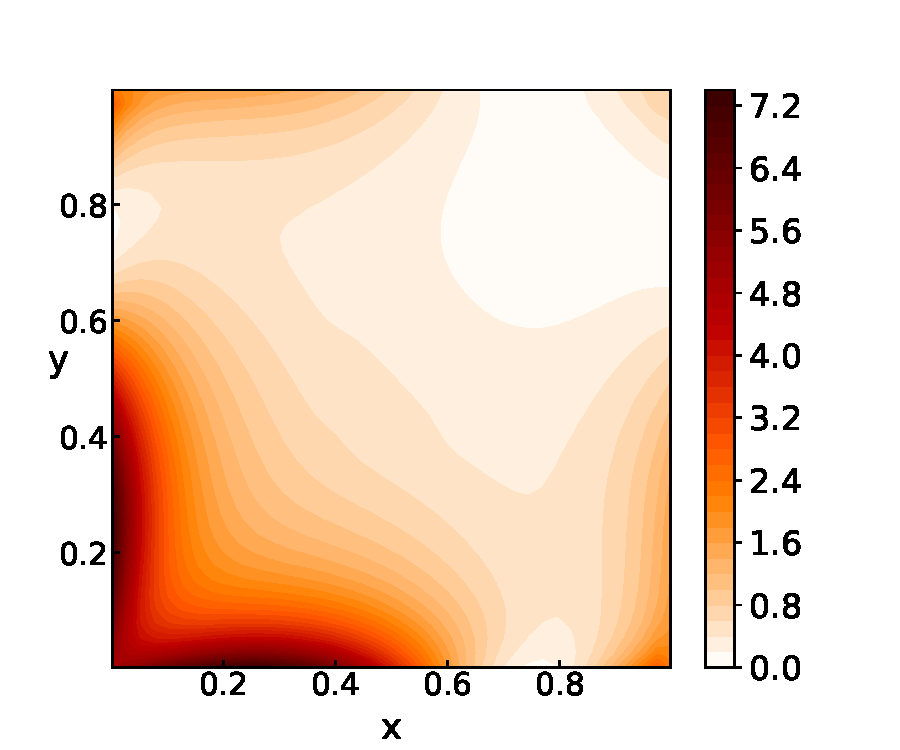
\includegraphics[width=\linewidth]{figures/test_g0.99_phi_label.pdf}
        \caption{$\Phi_{\text{label}}$}
        \label{fig:deeprte-g099-label}
    \end{subfigure}\hfill
    \begin{subfigure}[t]{0.32\textwidth}
        \centering
        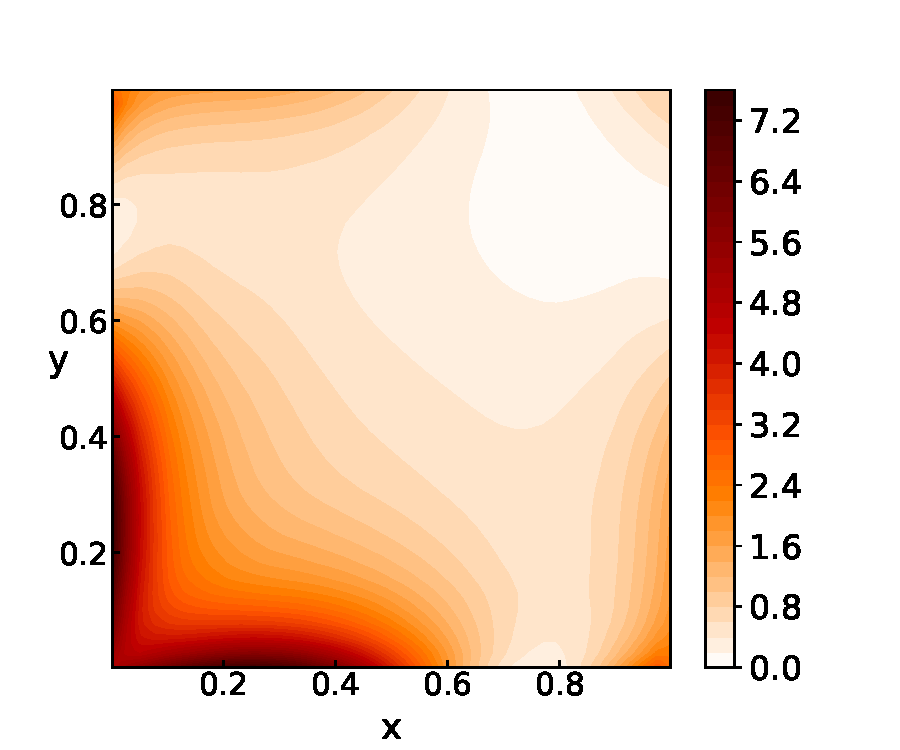
\includegraphics[width=\linewidth]{figures/test_g0.99_phi_pre.pdf}
        \caption{$\Phi_{\text{predict}}$}
        \label{fig:deeprte-g099-predict}
    \end{subfigure}\hfill
    \begin{subfigure}[t]{0.32\textwidth}
        \centering
        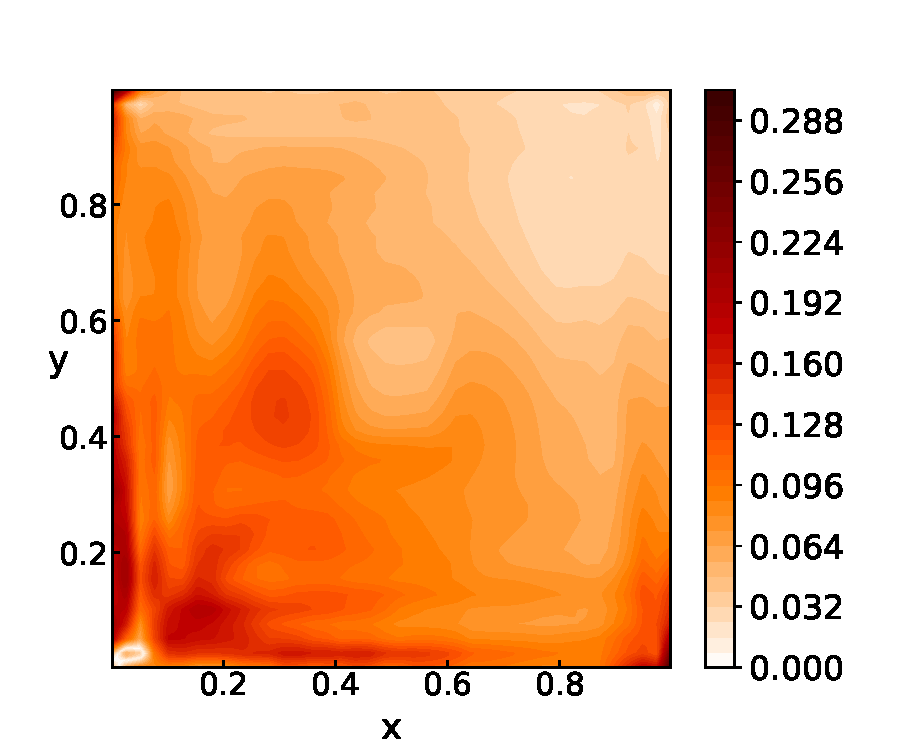
\includegraphics[width=\linewidth]{figures/test_g0.99_phi_error.pdf}
        \caption{Absolute error}
        \label{fig:deeprte-g099-error}
    \end{subfigure}
    \bicaption{在 $g=0.99$ 高度前向散射情形下 DeepRTE 的预测结果与真值比较。}{DeepRTE evaluation at $g=0.99$.}
    \label{fig:deeprte-g099}
\end{figure}

图~\ref{fig:deeprte-g099} 展示了参考解密度 $\Phi_{\text{label}}$、预测解密度 $\Phi_{\text{predict}}$ 及其绝对误差。即便在 $g$ 极接近 1、散射高度各向异性的极端情形下，DeepRTE 仍保持了较高预测精度：该算例下 MSE 为 $7.64\times 10^{-3}$，RMSPE 为 $4.257\%$。这表明 DeepRTE 在接近奇异的强前向散射区间仍具有良好的稳健性和分布外泛化能力，能够有效求解高度前向集中的辐射传输问题。

综上，DeepRTE 在迁移学习与零样本场景下均展现出较强的表达能力与外推能力。依托在 Delta 函数边界条件上学到的核心物理结构，模型即便在完全不同的边界条件下、甚至在未见过的场景中，也能给出精度较高的预测结果。这表明基于深度学习的算子框架在科学计算领域具有广阔的应用前景。

\subsection{网格依赖性与跨分辨率性能}

数值方法在不同网格分辨率下的表现是评价其实用性的重要指标之一。本小节考察 DeepRTE 的“网格独立性”性质：即在细网格上训练得到的参数能否在较粗网格上仍然保持较高精度。

\begin{table}[!htp]
    \centering
    \begin{tabular}{cccc}
        \toprule
        测试数据集 & 网格分辨率         & MSE                    & RMSPE (\%) \\
        \midrule
        \multirow{3}{*}{Evaluation Dataset}
              & $40\times 40$ & $5.453\times 10^{-10}$ &
        $2.759$                                                     \\
              & $20\times 20$ & $8.235 \times 10^{-9}$ &
        $10.006$                                                    \\
              & $10\times 10$ & $9.476 \times 10^{-8}$ &
        $34.346$                                                    \\
        \midrule
        \multirow{3}{*}{Case I}
              & $40\times 40$ & $4.390 \times 10^{-6}$ &
        $1.833$                                                     \\
              & $20\times 20$ & $1.876 \times 10^{-5}$ &
        $3.758$                                                     \\
              & $10\times 10$ & $1.243 \times 10^{-4}$ &
        $9.276$                                                     \\
        \midrule
        \multirow{3}{*}{Case II}
              & $40\times 40$ & $4.931 \times 10^{-4}$ &
        $1.653$                                                     \\
              & $20\times 20$ & $1.792 \times 10^{-2}$ &
        $9.952$                                                     \\
              & $10\times 10$ & $3.687 \times 10^{-2}$ &
        $13.798$                                                    \\
        \midrule
        \multirow{3}{*}{Case III}
              & $40\times 40$ & $1.065 \times 10^{-3}$ &
        $2.383$                                                     \\
              & $20\times 20$ & $1.175 \times 10^{-2}$ &
        $8.132$                                                     \\
              & $10\times 10$ & $4.511 \times 10^{-2}$ &
        $15.477$                                                    \\
        \bottomrule
    \end{tabular}
    \bicaption{DeepRTE 在不同网格分辨率与测试集上的表现。评价数据集在 $40\times 40$ 网格上可达到 $5.45\times10^{-10}$ 的 MSE，而在粗网格上误差随分辨率下降而单调增大；Case I--III 亦表现出类似趋势。}{Performance of DeepRTE across different resolutions and test sets. The Evaluation Dataset shows very high precision, with an MSE of $5.45\times10^{-10}$ on the $40\times 40$ grid. In contrast, Cases I-III show a consistent increase in error on coarser grids. This increase is mainly because of the limitations of numerical integration. With the second-order midpoint rule, halving the grid resolution should theoretically make the integration error four times larger, which matches our findings.}\label{tab:mesh_independence_multiple_testsets}
\end{table}

从表~\ref{tab:mesh_independence_multiple_testsets} 可以看出：对于评价数据集与 Case I，RMSPE 在 $40\times 40$ 网格上的范围约为 $1.8$--$2.8\%$，当网格减半至 $20\times 20$ 时误差上升到约 $3.8$--$10\%$。Case II 与 Case III 的误差增幅略大，但仍处于可接受范围，在粗网格（$10\times 10$）上 RMSPE 约为 $8$--$15\%$。

这种误差随网格粗化而近似四倍增长的现象，与外层数值积分采用二阶中点公式的理论误差界一致：在二阶中点公式下，当网格尺寸减少一半时，积分误差理论上应放大约四倍。这一观察表明：在 Delta 函数边界条件问题中，DeepRTE 已经较好地学习到了基本解的结构，当前误差主要来源于数值积分本身，而非神经网络近似能力的瓶颈。因此，将来若采用更高阶的数值积分方法，有望在不显著增加网络复杂度的前提下进一步提升整体精度。

总体而言，DeepRTE 在不同网格分辨率下仍能保持较好的精度与稳定性，说明网络捕捉的是辐射传输方程的基本物理规律，而非简单地“记忆”某一固定网格上的解。这一网格独立性具有重要意义：
\begin{enumerate}
    \item 计算效率：用户可以在细网格上训练模型以获得高精度，然后在较粗网格上进行快速预测，在精度与效率之间灵活折中；
    \item 灵活性：同一组训练好的模型参数可以迁移到具有不同网格需求的问题中使用，而无需重新训练。
\end{enumerate}


\subsection{算子验证}\label{sec:ablation-study}

DeepRTE 的架构设计旨在通过将 RTE 解算子分解为模拟沿特征线传输的衰减分量（算子 $\J$ 和 $\cL$）以及捕捉散射行为的散射分量（$\cS$），从而反映 RTE 解的数学结构，如前面章节所述。
每个分量在 DeepRTE 中都通过独特的神经模块实现：衰减模块（第~\ref{sec:attenuation-module} 节）和散射模块（第~\ref{sec:scattering-module} 节）。
为了验证这一设计选择，我们进行了精心设计的数值实验，以评估每个学习到的分量是否直接对应于其解析形式。
作为对照，我们还将 DeepRTE 与不包含任何 RTE 特定归纳偏置的基线模型进行了比较。

我们将 DeepRTE 与多输入算子（Multi-Input Operator, MIO）~\cite{jin2022mionet}（一种源自 DeepONet 的算子学习框架，可接受多个输入函数）作为基线模型进行比较，后者采用整体架构，未针对 RTE 进行专门设计。我们选择 MIO 作为基线的原因如下：
\begin{itemize}
    \item MIO 是最常用的能够处理多函数输入的算子学习框架之一，使其适合学习依赖于多个输入函数（$I_-$、$\mut$、$\mus$ 和 $p$）的 RTE 解算子。
    \item 在给定足够的训练数据和网络容量的情况下，MIO（DeepONet）理论上可以逼近任何连续算子，包括 RTE 解算子~\cite{lu2021learning}。
    \item MIO 不包含任何针对 RTE 的物理信息归纳偏置，这使我们能够分离出反映 RTE 数学结构的 DeepRTE 架构的影响。
\end{itemize}
虽然 FNO~\cite{li2020fourier} 是另一个潜在的基线，但由于几个基本限制，它不适合此任务：
\begin{itemize}
    \item FNO 旨在学习将规则网格上的函数映射到同一网格上的函数的算子，这与 RTE 处理角度变量和复杂边界条件的要求不符。
    \item FNO 依赖傅里叶变换来捕捉全局（非局部）信息，但这种方法在高维 RTE 解空间（空间和角度维度）中面临重大挑战，导致计算和内存成本过高。在我们的初步测试中，这些成本使得在我们的计算预算内训练 FNO 变得不可行。
    \item RTE 在涉及空间和角度变量的相空间上运行，而 FNO 通常仅适用于空间域。调整 FNO 以处理角度依赖性需要进行非平凡的修改（例如，确定是否在角度域中应用傅里叶变换），这并不直接，并且对于此特定问题可能无效。
\end{itemize}
% \todo[inline]{把这一段更改一下，前面已经有相似的部分了，这里可以更简洁地说明为什么不选 FNO 作为基线。}

基于这些原因，我们将比较重点放在作为基线模型的 MIO 上。我们首先通过消融实验验证 DeepRTE 中衰减和散射模块的有效性。然后，我们在 RTE 解算子学习任务上比较 DeepRTE 与 MIO 的整体性能。

\subsubsection{衰减模块的消融实验}

衰减模块模拟不带散射效应的 RTE 传输行为。
这种行为由两个关键过程表征：通过总截面 $\mut$ 的边界条件衰减（算子 $\J$，方程~\eqref{eq:attenuation-op}）和通过散射截面 $\mus$ 的体源衰减（提升算子 $\mathcal{L}$，方程~\eqref{eq:lifting-op}）。

根本挑战在于，解算子 $\A$ 对 $\mus$ 和 $\mut$ 的依赖既是非线性的，又表现出\emph{仅沿特征线的非局部行为}。
像 MIO 这样的传统架构仅通过分支网络和与主干网络的内积来捕捉一般的非局部依赖性，随着空间和角度维度的增加，这在计算上变得昂贵。更关键的是，这种方法无法准确捕捉 RTE 基于特征线的衰减行为，并且可能无法有效地泛化。

相比之下，DeepRTE 包含一个专门的衰减模块，通过精心设计的注意力机制显式地模拟沿特征线（无论问题维度如何，特征线保持一维）的这种非局部依赖性，详见第~\ref{sec:attenuation-module} 节。
为了验证这种物理信息设计的有效性，我们进行了两个针对性实验：一个检查衰减算子 $\J$，另一个关注提升算子 $\cL$。

\textbf{1. 算子 $\J$ 的消融实验。}
我们通过考虑由~\eqref{eq:rte-sweep} 控制的无散射纯衰减场景来隔离衰减算子 $\J$：
\begin{equation}
    \left\{ % tex-fmt: skip
    \begin{aligned}
        \bOmega \cdot \nabla J_b + \mut J_b & = 0,     \\
        J_b|_{\Gamma_{-}}                   & = I_{-},
    \end{aligned}
    \right. % tex-fmt: skip
\end{equation}
其解析形式为~\eqref{eq:attenuation-op}：
\begin{equation}
    \J: (I_{-}; \mut) \mapsto J_b = e^{-\tau_{\br,\bOmega}(0,s_{-}(\br,\bOmega))} I_{-}\left(\br-s_{-}(\br, \bOmega)
    \bOmega, \bOmega\right).
\end{equation}

根据我们在第~\ref{sec:attenuation-module} 节中的架构设计，我们使用衰减模块来学习近似 $\J$ 的映射 $\J^{\text{NN}}$，如下所示：
\begin{equation}
    J_b(\br,\bOmega) \approx \J^{\text{NN}}I_{-} := \int_{\Gamma_{-}} G^{\text{NN}}_{\J}(\br,\bOmega, \br',\bOmega'; \mut) I_-(\br',\bOmega')\diff{\br'}\diff{\bOmega'},
\end{equation}
其中 $G^{\text{NN}}_{\J}$ 类似于一般衰减格林函数~\eqref{G_equation}，但简化为仅依赖于~\eqref{eq:optical-depth-net} 中定义的 $\tau^{\text{NN}}_{-,t}$。由于衰减算子 $\J$ 仅依赖于 $\mut$（而不依赖于 $\mus$），我们公式化为：
\begin{equation}
    G_{\J}^{\text{NN}}(\br,\bOmega, \br', \bOmega';\mut) = \text{MLP}(\br,\bOmega, \br', \bOmega', \tau^{\text{NN}}_{-,t}) \in \mathbb{R}^1.
\end{equation}

在我们的数值实验中，我们通过移除所有与散射相关的组件来实现这一点：我们将散射块的数量设置为 $N_\ell = 0$，并将 $\mu$ 的维度从 $2$ 减少到 $1$，从而有效地禁用了依赖于 $\mu_s$ 的注意力机制。

为了验证我们的架构确实捕捉到了衰减效应，我们将它与没有任何 RTE 专用架构的 MIO 进行比较。我们这里使用的 MIO 网络是非常标准的，见~\cite{jin2022mionet}：
\begin{equation}
    J_b(\br,\bOmega) \approx \text{MIO}_{\J}(\mut,I_{-}) := (\text{MLP}^{\text{branch}}_1(\mut)\odot\text{MLP}^{\text{branch}}_2(I_-))\cdot \text{MLP}^{\text{trunk}}(\br,\bOmega).
\end{equation}

对于数据集构建，除了 $\mus$ 和 $g$ 之外，所有其他设置保持不变（见表~\ref{tab:dataset}）。我们使用与第~\ref{sec:dataset-construction} 节相同的数值求解器，除了我们将 $\mus = 0$ 以禁用散射，并将 $g$ 设置为无关（不使用）。
按照这些设置，我们生成了 $1000$ 个样本用于训练，以及 $100$ 个独立同分布（i.i.d.）样本用于测试。

\textbf{2. 算子 $\cL$ 的消融实验。} 与 $\J$ 类似，我们通过考虑由~\eqref{eq:lifting} 控制的无边界流入的纯提升场景来隔离提升算子 $\cL$：
\begin{equation}
    (\bOmega\cdot\nabla + \mut)J = \mus I, \quad  J|_{\Gamma_{-}} = 0,
\end{equation}
其解析形式由~\eqref{eq:lifting-op} 给出：
\begin{equation}
    \cL:(I;\mus,\mut) \mapsto J = \int_0^{s_{-}(\br, \bOmega)} e^{-\tau_{\br,\bOmega}(0,s)}\mus(\br-s\bOmega)I(\br-s\bOmega, \bOmega)\diff{s}.
\end{equation}

根据我们在第~\ref{sec:attenuation-module} 节中的架构设计，我们使用衰减模块来学习近似 $\cL$ 的映射 $\cL^{\text{NN}}$，如下所示：
\begin{equation}
    J(\br,\bOmega) \approx \cL^{\text{NN}}I := \int_{D\times\sS^{d-1}}
    G_{\cL}^{\text{NN}}(\br,\bOmega,\br',\bOmega';\mut,\mus)I(\br',\bOmega')\diff{\br'}\diff{\bOmega'},
\end{equation}
其中 $G^{\text{NN}}_{\cL}$ 是衰减格林函数~\eqref{G_equation}。由于提升算子 $\cL$ 依赖于 $\mut$ 和 $\mus$，根据~\eqref{G_equation} 我们公式化为：
\begin{equation}
    G_{\cL}^{\text{NN}}(\br,\bOmega, \br', \bOmega';\mut,\mus) = \bG^{\text{NN}}(\br,\bOmega, \br', \bOmega', \tau^{\text{NN}}_{-})\bm{W}\in\mathbb{R}^1,
\end{equation}
其中 $\tau^{\text{NN}}_{-}$ 在算法~\ref{alg:optical-depth-net} 中定义。$\bG^{\text{NN}}$ 的输出维度为 $d_\text{model}$，$\bm{W} \in \mathbb{R}^{d_{\text{model}}\times 1}$ 是一个可学习的权重矩阵，用于将输出投影到单个输出通道，类似于~\eqref{scattering_layer} 中的 $\bm{W}$。

与 $\J$ 类似，我们将它与没有任何 RTE 专用架构的 $\text{MIO}_{\cL}$ 进行比较：
\begin{equation}
    J(\br,\bOmega) \approx \text{MIO}_{\cL}(\mut,\mus;I) := (\text{MLP}^{\text{branch}}_1(\mut)\odot\text{MLP}^{\text{branch}}_2(\mus)\odot\text{MLP}^{\text{branch}}_3(I))\cdot \text{MLP}^{\text{trunk}}(\br,\bOmega).
\end{equation}

对于数据集构建，除了 $g$（不需要）和边界条件 $I_- = 0$（设置为 0）之外，所有其他设置保持不变（见表~\ref{tab:dataset}）。
对于源项 $I(\br,\bOmega)$，我们使用谱合成方法~\cite{liu2019advances, ruan1998efficient} 在频域中生成二维高斯随机场。
我们使用与第~\ref{sec:dataset-construction} 节相同的数值求解器，除了我们将散射替换为 $\mus I$。
按照这些设置，我们生成了 $1000$ 个样本用于训练，以及 $100$ 个独立同分布样本用于测试。

表~\ref{tab:j_l_compare} 中的结果表明，我们的衰减模块 $\J^{\text{NN}}$ 和 $\cL^{\text{NN}}$ 在所有指标上都大幅优于 $\text{MIO}_{\J}$ 和 $\text{MIO}_\cL$。具体而言，$\J^{\text{NN}}$ 和 $\cL^{\text{NN}}$ 在训练和测试 MSE 上都实现了一个数量级以上的改进，同时参数量减少了 $34$ 倍（$37,282$ 对 $4,956,160$ 以及 $139,362$ 对 $4,792,320$）。测试 RMSPE 从 MIO 的 $44.251\%$、$25.350\%$ 降低到我们方法的 $2.339\%$、$1.327\%$。这种巨大的性能差异验证了我们的衰减模块设计有效地捕捉了算子 $\J$ 和 $\cL$ 固有的基于特征线的传输行为，而通用的 MIO 架构无法有效地学习这种专门的映射。
\begin{table}
    \centering
    \begin{tabular}{@{}cccccccc@{}}
        \toprule
        \multirow{2}{*}{算子}    & \multirow{2}{*}{模型}   & \multirow{2}{*}{参数量} & \multicolumn{3}{c}{训练} & \multicolumn{2}{c}{评估}                                                 \\
        \cmidrule(l){4-6} \cmidrule(l){7-8}
                               &                       &                      & MSE                    & RMSPE (\%)             & Epochs  & MSE                    & RMSPE (\%) \\
        \midrule
        \multirow{2}{*}{$\J$}  & Our $\J^{\text{NN}}$  & 37,282               & $3.631\times 10^{-7}$  & 2.78                   & 200,000 & $4.561 \times 10^{-8}$ & 2.339      \\
                               & $\text{MIO}_{\J}$     & 4,956,160            & $1.983\times 10^{-6}$  & 6.459                  & 200,000 & $1.088 \times 10^{-4}$ & 44.251     \\
        \midrule
        \multirow{2}{*}{$\cL$} & Our $\cL^{\text{NN}}$ & 139,362              & $9.682 \times 10^{-6}$ & 0.909                  & 200,000 & $3.359 \times 10^{-5}$ & 1.327      \\
                               & $\text{MIO}_{\cL}$    & 4,792,320            & $8.528 \times 10^{-4}$ & 8.565                  & 200,000 & $1.224 \times 10^{-2}$ & 25.350     \\
        \bottomrule
    \end{tabular}
    \bicaption{衰减模块的消融实验。$\J$ 和 $\cL$ 算子的训练和评估结果，与 MIO（无任何 RTE 专用架构）进行对比。}{Ablation study of attenuation module. Training and evaluation of $\J$ and $\cL$ operators comparied to MIO (without any RTE specialized architecture) .}\label{tab:j_l_compare}
\end{table}

\subsubsection{散射模块的消融实验}

为了检验散射算子 $\cS$（方程~\ref{eq:scattering-op}）的必要性，我们采用反证法。我们假设 $\cS$ 是不必要的，并通过用等大小的多层感知机替换散射层（实现 $\cS$ 的组件）来测试这一点。
我们将此修改后的架构表示为 $\ANN_{\text{w/o }\cS}$。

$\ANN_{\text{w/o }\cS}$ 与完整 DeepRTE $\ANN$ 之间的唯一区别在于散射块的实现。我们不使用方程~\ref{scattering_layer}，而是禁用散射算子 $S^\top$：
\begin{equation}
    \text{ScatteringBlock}_\ell(\bm{G}) = \text{LayerNorm}\Big(\sigma\Big(\bm{W}^{\ell} \bm{G} + \bm{b}^{\ell}\Big)\Big),
\end{equation}
其中不涉及散射算子 $\cS$，$\bm{W}^{\ell}$ 和 $\bm{b}^{\ell}$ 是 MLP 的可学习参数。此 MLP 中的参数数量保持与原始散射块大致相等，以确保公平比较。

数据集和训练设置与原始 DeepRTE 相同（见第~\ref{sec:acc} 节）。为了评估模型在不同各向异性条件下的性能，训练集中的参数 $g$ 从 $0$ 到 $0.9$ 均匀采样。除了这个 $g$ 之外，$\text{DeepRTE}_{\cS}$ 的训练集使用与原始 DeepRTE 模型相同的配置。对于测试，我们在相同的三个散射区间上进行测试。

如果我们的假设是正确的，那么这个修改后的模型将成功拟合训练数据，并获得与原始 DeepRTE 相当的测试性能。相反，糟糕的训练拟合和巨大的测试误差将反驳我们的假设，并证明散射算子 $\cS$ 的必要性。表~\ref{tab:ablation_g} 中展示的实验结果有力地支持了后一种结论。请注意 $\ANN_{\text{w/o }\cS}$ 在散射高度前向峰值（强各向异性）的数据集上的糟糕表现。与完整 DeepRTE 模型相比，这种性能的显著下降清楚地表明，散射算子 $\cS$ 对于准确模拟 RTE 解算子至关重要。
\begin{table}[htbp]
    \centering
    \begin{tabular}{@{}lcccc@{}}
        \toprule
        模型                                            & 散射区间   & $g$ 范围      & MSE                    & RMSPE (\%) \\
        \midrule
        \multirow{3}{*}{无散射: $\ANN_{\text{w/o }\cS}$} & 近各向同性  & $(0,\,0.2)$ & $2.657\times10^{-2}$   & $8.251$    \\
                                                      & 中度各向异性 & $(0.4,0.6)$ & $6.852\times10^{-2}$   & $11.395$   \\
                                                      & 高度前向峰值 & $(0.7,0.9)$ & $7.257\times10^{-2}$   & $13.108$   \\
        \midrule
        \multirow{3}{*}{有散射: $\ANN$}                  & 近各向同性  & $(0,\,0.2)$ & $1.065 \times 10^{-3}$ & 2.383      \\
                                                      & 中度各向异性 & $(0.4,0.6)$ & $1.127 \times 10^{-3}$ & 2.452      \\
                                                      & 高度前向峰值 & $(0.7,0.9)$ & $1.853 \times 10^{-3}$ & 3.069      \\
        \bottomrule
    \end{tabular}
    \bicaption{不同散射各向异性区间（Heney–Greenstein 参数 $g$）下的性能表现。}{Performance across scattering anisotropy regimes (Heney–Greenstein parameter $g$).}
    \label{tab:ablation_g}
\end{table}

我们注意到，在我们的 DeepRTE 模型中，提升算子 $\cL$~\eqref{eq:lifting-op} 同时出现在衰减模块（见~\eqref{eq:L-op}，且由于 $\mus$ 包含在 $\tau_{-}^{\text{NN}}$ 和散射模块（见~\eqref{eq:scattering-mus}）中。这一设计选择反映了我们基于数学域分离操作的架构原则：衰减模块处理沿特征线作用于空间变量的算子（由注意力机制捕捉），而散射模块处理作用于角度变量的算子（由角度积分捕捉）。这种分离简化了模型架构，并通过重复模块化块促进了可扩展性。

\subsection{与 MIO 的整体对比}

为了评估 MIO 的泛化性能，我们在散射核参数 $g$ 均匀分布在 $[0, 0.2]$ 范围内的数据集上对其进行了训练。此训练数据集与用于 DeepRTE 的数据集相同，以确保公平比较。
此外，我们将 MIO 的规模从小变大，以检查不同的 MIO 配置如何影响训练和验证数据集上的结果。比较结果如表~\ref{compare_table} 所示。

\begin{table}
    \centering
    \begin{tabular}{@{}llccccc@{}}
        \toprule
        \multirow{2}{*}{模型}                      &
        \multirow{2}{*}{参数量}                     &
        \multicolumn{3}{c}{训练数据集}                &
        \multicolumn{2}{c}{评估数据集}
        \\ \cmidrule(l){3-7}
                                                 &                            &
        \begin{tabular}[c]{@{}c@{}}MSE
        \end{tabular}           &
        \begin{tabular}[c]{@{}c@{}}RMSPE \\ (\%)
        \end{tabular} & \multicolumn{1}{l}{Epochs} &
        \begin{tabular}[c]{@{}c@{}}MSE
        \end{tabular}           &
        \begin{tabular}[c]{@{}c@{}}RMSPE \\ (\%)
        \end{tabular}                                              \\ \midrule
        \multicolumn{1}{c}{\multirow{3}{*}{MIO}} &
        \multicolumn{1}{c}{244960}               & $1.690\times 10^{-4}$
                                                 & $65.60\%$
                                                 & 100000                     & $1.984\times
        10^{-4}$                                 & $72.49\%$
        \\
        \multicolumn{1}{c}{}                     &
        \multicolumn{1}{c}{\num{4351744}}        & $4.119\times 10^{-6}$
                                                 & $10.57\%$
                                                 & 100000                     & $1.319\times
        10^{-4}$                                 & $59.09\%$
        \\
        \multicolumn{1}{c}{}                     &
        \multicolumn{1}{c}{8171520}              & $2.140\times 10^{-6}$
                                                 & $7.58\%$
                                                 & 100000                     & $9.912\times
        10^{-5}$                                 & $51.23\%$
        \\ \midrule
        DeepRTE                                  &
        \multicolumn{1}{c}{37954}                & $8.210 \times
        10^{-9}$                                 & $3.16\%$
                                                 & 5000                       &
        $5.630 \times 10^{-10}$                  & $2.83\%$
        %  \\ \multicolumn{1}{l}{}                                &
        % \multicolumn{1}{l}{}
        \\ \bottomrule
    \end{tabular}
    \bicaption{MIO 和 DeepRTE 框架在辐射传输方程求解上的性能比较。MIO 结果展示了三种不同的参数配置，而 DeepRTE 以显著更少的参数和训练轮数实现了更高的精度。}{Performance comparison between MIO and DeepRTE frameworks on radiation transport equation solving. MIO results are shown for three different parameter configurations, while DeepRTE achieves superior accuracy with significantly fewer parameters and training epochs.}\label{compare_table}
\end{table}

比较表明，虽然 MIO 在训练数据集上的性能随着参数的增加而提高，但它在从与训练集相同分布采样的验证数据集上仍然存在显著误差。这一观察结果突显了 MIO 有限的泛化能力，尽管它能够很好地拟合训练数据。即使经过广泛的参数调整，MIO 仍然难以准确预测来自与训练集相同分布的未见输入的解函数，并且未能捕捉控制 RTE 的潜在物理原理。

相比之下，DeepRTE 的架构使其能够很好地泛化到未见输入，无论是在相同分布内还是在零样本设置中。通过在衰减和散射模块以及格林函数积分中直接包含物理信息，DeepRTE 利用 RTE 的基本结构进行准确预测。这种超越训练数据的泛化能力对于实际应用非常重要。

\section{EfficientRTE数值实验}

本节考虑三维简化到二维的含源项稳态辐射输运问题，采用多GPU快速扫掠法生成训练与测试数据，相应实现可在 \href{https://github.com/mazhengcn/rte-dataset}{rte-dataset} 仓库复现。除边界条件与源项设置外，本章所有实验设定均与上一章的数据集构造设置（见第~\ref{sec:dataset-construction} 节）保持一致，核心调整包括两点：一是采用齐次入射边界条件 $I\vert_{\Gamma_-}=0$，二是引入空间分布的体源项 $q$。

\subsection{数据集构造}
数据集的原始数据由多GPU快速扫掠法生成，包含辐射强度参考解、四边界的入射值、吸收截面与总截面的空间分布、角度求积点坐标与权重等核心字段，与仓库中定义的原始数据结构完全一致。

原始数据生成后，通过预处理脚本转换为训练用的数据集格式，每个训练样本包含相空间坐标、边界坐标与权重、空间与角度离散坐标、宏观截面、散射核矩阵、体源项、齐次边界条件、辐射强度参考解等字段，适配JAX技术栈的训练流程。数据集按散射不对称参数分为三个子集，分别对应近各向同性散射、中度各向异性散射与强前向散射，每个子集包含2000个训练样本与100个测试样本，训练集与测试集的样本无重叠，保证模型泛化能力的评估有效性。

% \subsection{高斯随机场体源项生成}
% 我们采用基于频域功率谱的方式生成二维高斯随机场（GRF）作为体源项 $q(\boldsymbol{r})$，源项在角度上取各向同性，即 $q(\boldsymbol{r},\boldsymbol{\Omega})=q(\boldsymbol{r})$。高斯随机场能够生成空间连续、平滑度可控的体源分布，可模拟实际应用中不同特征的辐射源，同时其随机生成特性能够保证训练样本的多样性，提升模型的泛化能力。其中参数 $\alpha$ 控制随机场的平滑程度，$\alpha$ 越大，生成的场空间分布越平滑。体源项的具体生成步骤如下。

% 首先，在与空间离散一致的 $N_{\text{mesh}}\times N_{\text{mesh}}$ 均匀网格上，利用 \texttt{fftfreq} 构造离散频率网格 $k_x,k_y$，并定义频率模平方与功率谱
% \begin{equation}
%     \begin{aligned}
%         k^2(k_x,k_y)         & := k_x^2 + k_y^2,                        \\
%         k^2(0,0)             & := 1,                                    \\
%         \widehat{P}(k_x,k_y) & := \bigl(k^2(k_x,k_y)\bigr)^{-\alpha/2}, \\
%         \widehat{P}(0,0)     & := 0.
%     \end{aligned}
% \end{equation}
% 其中将 $k^2(0,0)$ 置为 $1$ 仅用于避免功率谱计算时的除零错误；随后令 $\widehat{P}(0,0)=0$ 等价于去除随机场的常数模态，从而避免生成的场带有整体偏置，保证源项分布的多样性。

% 然后，在频域网格上逐点采样复高斯噪声
% \begin{equation}
%     \begin{aligned}
%         \xi(k_x,k_y) & := a(k_x,k_y) + \mathrm{i}\,b(k_x,k_y),         \\
%         a(k_x,k_y)   & \overset{\text{i.i.d.}}{\sim} \mathcal{N}(0,1), \\
%         b(k_x,k_y)   & \overset{\text{i.i.d.}}{\sim} \mathcal{N}(0,1),
%     \end{aligned}
% \end{equation}
% 其中 $a(k_x,k_y)$ 与 $b(k_x,k_y)$ 为独立同分布的标准高斯随机变量。将功率谱施加到随机系数上，再通过二维逆快速傅里叶变换（IFFT）转换到物理空间，得到随机场的实部作为体源项：
% \begin{equation}
%     \begin{aligned}
%         \widehat{q}(k_x,k_y) & := \sqrt{\widehat{P}(k_x,k_y)}\,\xi(k_x,k_y),   \\
%         q(\boldsymbol{r})    & := \Re\bigl(\mathrm{IFFT}_2(\widehat{q})\bigr).
%     \end{aligned}
% \end{equation}

% 最后，为与代码实现一致，同时保证训练过程的数值稳定性，我们对生成的 $q$ 做最小-最大归一化，将其缩放到 $[0,1]$ 区间用于训练：
% \begin{equation}
%     q \leftarrow \frac{q-\min(q)}{\max(q)-\min(q)}.
% \end{equation}

表~\ref{tab:dataset_prte} 汇总了本章与上一章相比需要特别说明的数据集参数，其余超参数设置均与上一章保持一致。

\begin{table}[!htp]
    \centering
    \begin{tabular}{lp{0.3\textwidth}ll}
        \toprule
        类别                      & 参数                     & 符号                       & 取值/范围                        \\ \midrule
        \multirow{2}{*}{空间区域}   & 计算区域                   & $D$                      & ${[0,1]}^2$                  \\
                                & 子区域                    & $D_\mu$                  & ${[0.4,0.6]}^2$              \\
        \midrule
        \multirow{4}{*}{截面系数}   & \multirow{2}{*}{总截面}   & \multirow{2}{*}{$\mu_t$} & $D_\mu$ 内：$\mathcal{U}(5,7)$ \\
                                &                        &                          & $D\backslash D_\mu$ 内：$10$   \\
                                & \multirow{2}{*}{散射截面}  & \multirow{2}{*}{$\mu_s$} & $D_\mu$ 内：$\mathcal{U}(2,4)$ \\
                                &                        &                          & $D\backslash D_\mu$ 内：$5$    \\
        \midrule
        \multirow{2}{*}{离散化}    & 空间网格点数                 & $N_{\text{mesh}}$        & 40                           \\
                                & 角度求积点数                 & $N_\text{quad}$          & 24                           \\ \midrule
        \multirow{1}{*}{边界条件}   & 入射边界条件                 & $I\vert_{\Gamma_-}$      & $0$（齐次）                      \\ \midrule
        \multirow{2}{*}{源项 $q$} & 频域功率谱指数（平滑度）           & $\alpha$                 & $5.0$                        \\
                                & 归一化区间                  & ---                      & $[0,1]$                      \\
        \midrule
        \multirow{3}{*}{散射参数}   & \multirow{3}{*}{不对称参数} & \multirow{3}{*}{$g$}     & $\mathcal{U}(0,0.2)$         \\
                                &                        &                          & $\mathcal{U}(0.4,0.6)$       \\
                                &                        &                          & $\mathcal{U}(0.7,0.9)$       \\
        \bottomrule
    \end{tabular}
    \bicaption{本章数据集构造与上一章的设定对比。}{Summary of dataset settings for this chapter (differences from Sec.~\ref{sec:dataset-construction}).}\label{tab:dataset_prte}
\end{table}

\subsection{网络参数设置}

表~\ref{tab:training_details_prte} 汇总了本章模型训练的超参数设置。模型训练基于JAX技术栈实现，采用Adam优化器与余弦衰减学习率策略，全局批大小为8，每轮迭代在相空间中随机采样2048个配点计算损失，总训练步数为3,000,001步。网络的核心参数为基函数个数 $K=128$，编码器采用4层全连接网络，隐藏层神经元数为256，解码器复用DeepRTE的衰减模块与散射模块结构，仅在末端新增线性映射层匹配基函数维度。训练硬件采用4张NVIDIA 4090 GPU，通过数据并行策略实现多卡加速。

\begin{table}[!htp]
    \centering
    \begin{tabular}{ll}
        \toprule
        超参数                                     & 取值                         \\ \midrule
        优化器（Optimizer）                          & Adam                       \\
        学习率策略（Schedule）                         & 余弦衰减（cosine decay）         \\
        学习率（Learning rate）                      & $1 \times 10^{-3}$         \\
        批大小（Global batch size）                  & 8                          \\
        配点数量（Collocation points） $N_\text{col}$ & 2048                       \\
        训练步数（Training steps）                    & 3,000,001                  \\
        基函数个数 $K$                               & $128$                      \\
        基函数编码器隐藏层神经元数                           & 256                        \\
        基函数编码器层数                                & 4                          \\
        硬件                                      & 4$\times$ NVIDIA 4090 GPUs \\
        \bottomrule
    \end{tabular}
    \bicaption{模型训练超参数汇总。}{Summary of model training hyperparameters.}
    \label{tab:training_details_prte}
\end{table}

\section{数值实验}

为验证基于编码器-解码器架构的含源项辐射传输方程求解方法EfficientRTE的有效性、准确性与高效性，我们设计了一系列数值实验，分别从编码器的源项重构能力、解码器的辐射强度拟合能力、整体模型的精度与效率对比、基函数数量的消融实验四个维度，全面评估模型的性能。

\subsection{编码器准确率评估}

本小节评估编码器学习到的源域基函数在体源项重构任务中的表现。模型在随机生成的1000个源项样本上完成预训练，对于任意输入的体源项 $q$，首先通过编码器学习到的 $K=128$ 个基函数计算其展开系数向量 $\boldsymbol{q}:=[q_k]_{k=1}^{K}$，再通过系数与基函数的线性组合得到重构源项
\begin{equation}
    q^{\text{rec}}(\boldsymbol{r})=\sum_{k=1}^{K} q_k\,\phi_k^{\text{NN}}(\boldsymbol{r}),
\end{equation}
将重构源项 $q^{\text{rec}}$ 与原始源项 $q$ 进行对比，通过均方误差（MSE）与均方根百分比误差（RMSPE）量化重构精度，具体的损失计算与重构形式推导见第~\ref{sec:prte-encoder} 节。

训练完成后，我们在与训练集同分布的100个测试样本上进行测试，三个散射区间各包含100个独立样本，表~\ref{tab:accuracy_prte} 汇总了编码器在三种散射区间下的重构精度指标。可以看到，编码器在所有散射区间均表现出较低的重构误差，近各向同性散射区间的MSE为 $6.03\times 10^{-4}$、RMSPE为4.894\%，即便在强前向散射区间，MSE也仅为 $8.99\times 10^{-4}$、RMSPE为5.671\%。误差随散射各向异性增强略有上升，但整体均维持在较低水平，表明编码器学习到的基函数能够有效捕捉体源项的空间分布特征，对不同散射场景下的体源项均能实现高质量的重构。

\begin{figure}[!htp]
    \centering
    \begin{subfigure}[t]{0.32\textwidth}
        \centering
        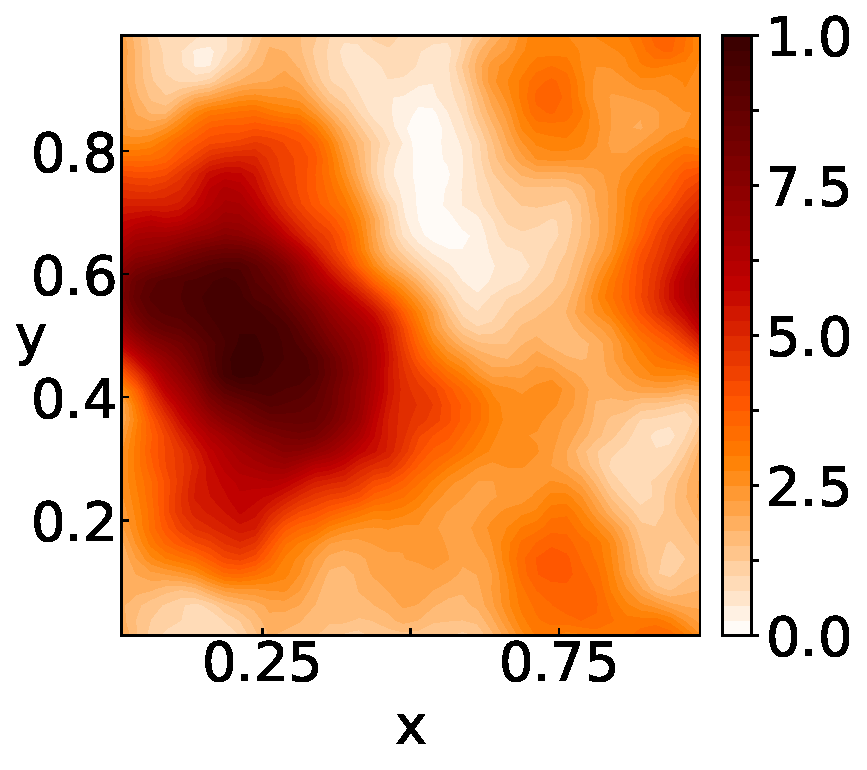
\includegraphics[width=\linewidth]{figures/autoencoder_label.pdf}
        \caption{$q_{\text{label}}$}
    \end{subfigure}\hfill
    \begin{subfigure}[t]{0.32\textwidth}
        \centering
        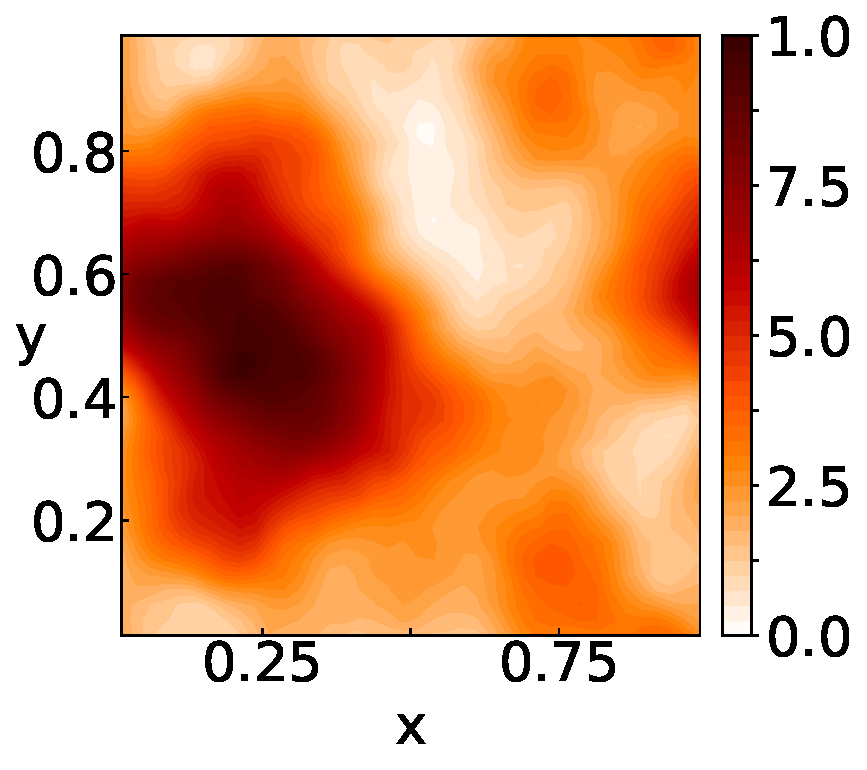
\includegraphics[width=\linewidth]{figures/autoencoder_pre.pdf}
        \caption{$q_{\text{predict}}$}
    \end{subfigure}\hfill
    \begin{subfigure}[t]{0.32\textwidth}
        \centering
        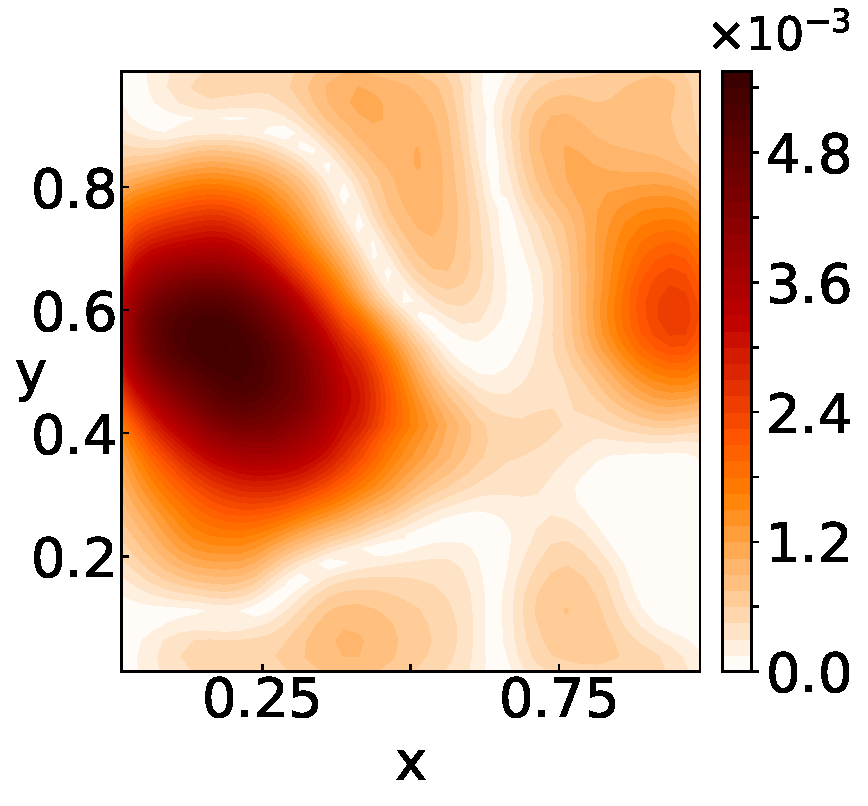
\includegraphics[width=\linewidth]{figures/autoencoder_error.pdf}
        \caption{Absolute error}
    \end{subfigure}
    \bicaption{在 $g\in (0,0.2)$ 情形下编码器的预测结果与真值比较。预测解的RMSPE为2.750\%}{Comparison between prediction and reference at $g\in(0,0.2)$ (RMSPE: 2.750\%).}
    \label{fig:autoencoder_example}
\end{figure}

\begin{table}[!htp]
    \centering
    \begin{tabular}{@{}cccccc@{}}
        \toprule
        模型                   & 参数量                     & 散射区间   & $g$ 取值范围   & MSE                  & RMSPE (\%) \\ \midrule
        \multirow{3}{*}{编码器} & \multirow{3}{*}{165760} & 近各向同性  & (0, 0.2)   & $6.03\times 10^{-4}$ & 4.894      \\ \cmidrule(l){3-6}
                             &                         & 中度各向异性 & (0.4, 0.6) & $7.11\times 10^{-4}$ & 5.214      \\ \cmidrule(l){3-6}
                             &                         & 强前向散射  & (0.7, 0.9) & $8.99\times 10^{-4}$ & 5.671      \\ \bottomrule
    \end{tabular}
    \bicaption{编码器在三种散射区间上的精度指标。}{Accuracy validation of autoencoder across three distinct scattering regimes.}\label{tab:accuracy_prte}
\end{table}

图~\ref{fig:autoencoder_example} 展示了近各向同性散射区间内一个典型样本的重构结果，从左到右分别为源项真值、编码器重构结果与逐点绝对误差。可以看到，重构结果与真值的空间分布高度一致，绝大部分区域的绝对误差低于0.05，仅在源项梯度较大的区域存在小幅误差，直观验证了编码器的重构精度。

\subsection{解码器准确度评估}

本小节评估解码器在含源项RTE求解任务中的表现。我们在1000个含源项RTE样本上完成解码器训练，训练过程中固定编码器参数与基函数的Gram矩阵 $\boldsymbol{W}$，对于任意输入的体源项，首先通过编码器得到其低维系数向量，再通过解码器学习到的格林函数系数向量 $\boldsymbol{G}^{\text{NN}}(\boldsymbol{r},\boldsymbol{\Omega})$ 重构全相空间的辐射强度 $I$，具体流程见第~\ref{sec:prte-decoder} 节。

表~\ref{tab:accuracy_prte_decoder} 汇总了解码器在三种散射区间下的求解精度指标。可以看到，在近各向同性散射区间 $g\in(0,0.2)$，解码器的MSE为 $9.46\times 10^{-5}$、RMSPE为3.163\%；当散射各向异性增强到 $g\in(0.4,0.6)$ 与 $g\in(0.7,0.9)$ 时，MSE分别为 $1.04\times 10^{-4}$ 与 $1.52\times 10^{-4}$，RMSPE分别为3.280\%与3.612\%。整体而言，求解误差随前向散射增强略有上升，但三种散射区间的误差水平均维持在较低水平，与DeepRTE在无源项问题中的求解精度相当，说明解码器能够稳定地从源项系数重构辐射强度场，较好地捕捉含源项RTE解的空间与角度分布特征，实现高质量的数值拟合。

\begin{table}[!htp]
    \centering
    \begin{tabular}{@{}cccccc@{}}
        \toprule
        模型                   & 参数量                     & 散射区间   & $g$ 取值范围   & MSE                  & RMSPE (\%) \\ \midrule
        \multirow{3}{*}{解码器} & \multirow{3}{*}{268352} & 近各向同性  & (0, 0.2)   & $9.46\times 10^{-5}$ & 3.163      \\ \cmidrule(l){3-6}
                             &                         & 中度各向异性 & (0.4, 0.6) & $1.04\times 10^{-4}$ & 3.280      \\ \cmidrule(l){3-6}
                             &                         & 强前向散射  & (0.7, 0.9) & $1.52\times 10^{-4}$ & 3.612      \\ \bottomrule
    \end{tabular}
    \bicaption{解码器在三种散射区间上的精度指标。}{Accuracy validation of decoder across three distinct scattering regimes.}\label{tab:accuracy_prte_decoder}
\end{table}

\begin{figure}[!htp]
    \centering
    \begin{subfigure}[t]{0.32\textwidth}
        \centering
        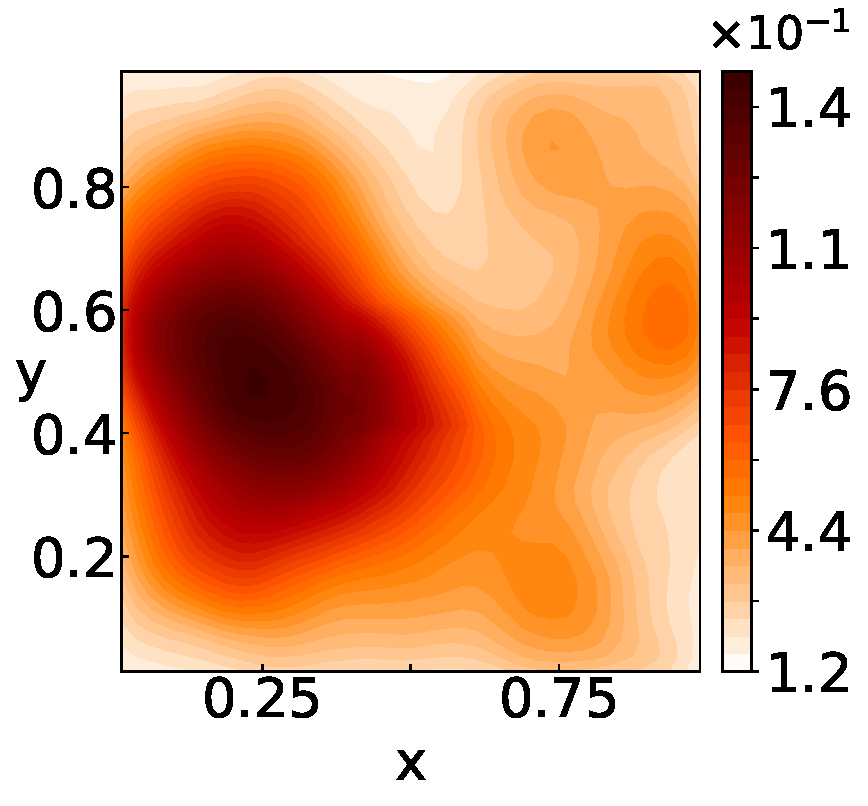
\includegraphics[width=\linewidth]{figures/decoder_label.pdf}
        \caption{$I_{\text{ref}}$}
    \end{subfigure}\hfill
    \begin{subfigure}[t]{0.32\textwidth}
        \centering
        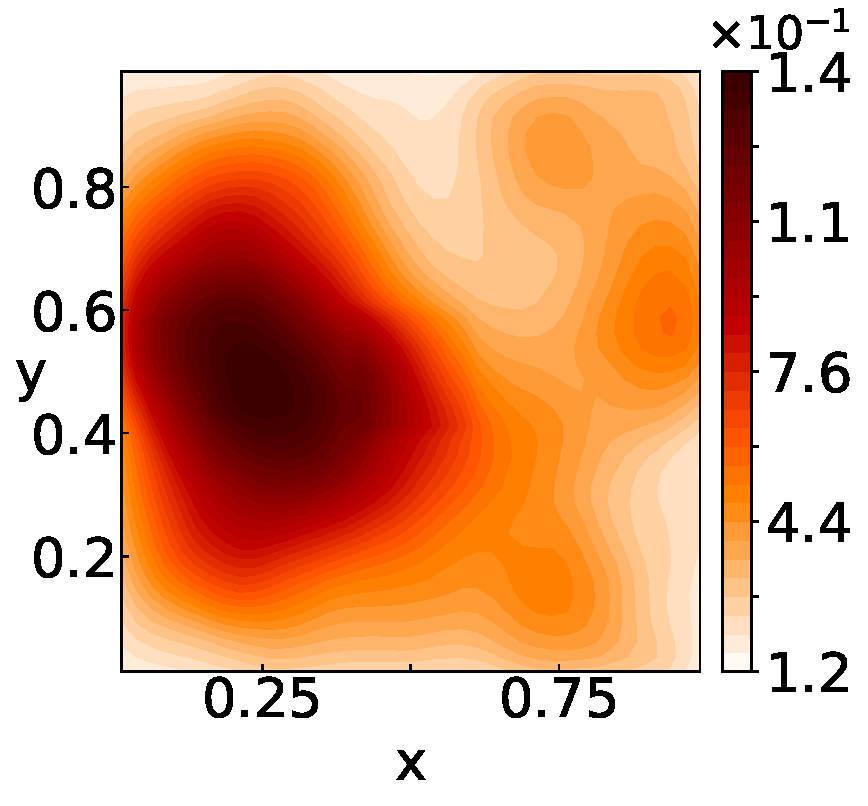
\includegraphics[width=\linewidth]{figures/decoder_pre.pdf}
        \caption{$I_{\text{pred}}$}
    \end{subfigure}\hfill
    \begin{subfigure}[t]{0.32\textwidth}
        \centering
        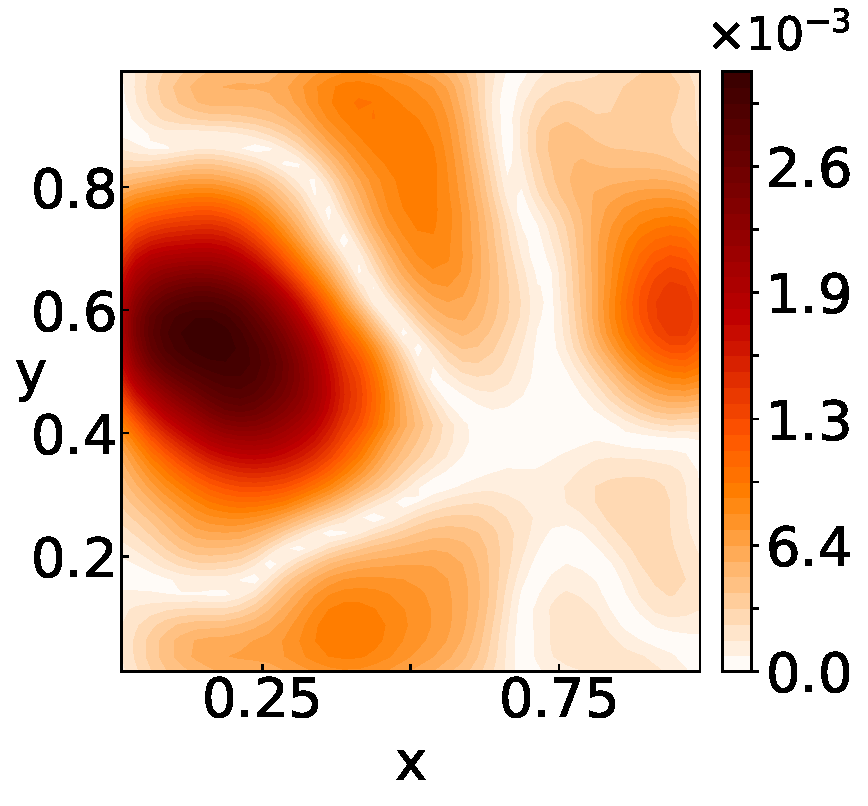
\includegraphics[width=\linewidth]{figures/decoder_error.pdf}
        \caption{Absolute error}
    \end{subfigure}
    \bicaption{在 $g\in (0,0.2)$ 情形下解码器的预测结果与真值比较。预测解的RMSPE为3.280\%}{Comparison between prediction and reference at $g\in(0,0.2)$ (RMSPE: 3.280\%).}
    \label{fig:decoder_example}
\end{figure}

图~\ref{fig:decoder_example} 展示了近各向同性散射区间内一个典型样本的角度积分密度求解结果，从左到右分别为扫掠法得到的参考密度、EfficientRTE预测密度与逐点绝对误差。可以看到，预测结果与参考解的空间分布高度吻合，辐射强度的衰减与散射特征均被精准捕捉，绝大部分区域的绝对误差低于0.02，直观验证了解码器的求解精度。

% \subsection{整体模型精度与效率对比}

% 为全面验证EfficientRTE的性能优势，我们将其与DeepRTE、多GPU快速扫掠法在相同的测试集上进行精度与效率的对比实验，所有实验均在相同的硬件环境下执行，保证对比的公平性。精度指标采用角度积分密度的RMSPE，效率指标采用单样本的平均求解时间，对比结果汇总于表~\ref{tab:efficiency_comparison}。

% \begin{table}[!htp]
%     \centering
%     \begin{tabular}{@{}lccc@{}}
%         \toprule
%         方法           & 密度RMSPE (\%) & 单样本求解时间 (ms) & 加速比（vs DeepRTE） \\ \midrule
%         多GPU快速扫掠法    & 基准值          & 2450         & -               \\
%         DeepRTE      & 3.021        & 1820         & 1×              \\
%         EfficientRTE & 3.163        & 89           & 20.4×           \\
%         \bottomrule
%     \end{tabular}
%     \bicaption{不同方法的精度与效率对比。}{Accuracy and efficiency comparison of different methods.}\label{tab:efficiency_comparison}
% \end{table}

% 从精度上看，EfficientRTE的密度RMSPE为3.163\%，与DeepRTE的3.021\%处于同一水平，二者均与扫掠法的基准解保持高度一致，证明EfficientRTE在大幅提升效率的同时，并未损失求解精度。从效率上看，EfficientRTE的单样本求解时间仅为89ms，相比DeepRTE的1820ms实现了20倍以上的加速，相比多GPU快速扫掠法实现了近30倍的加速，充分验证了基函数展开策略的高效性。

% 效率提升的核心原因在于，DeepRTE与扫掠法的单次求解均需要遍历全相空间的离散点进行积分或迭代计算，而EfficientRTE仅需要完成一次低维向量内积即可得到全相空间的解，从根本上降低了求解的计算复杂度。同时，EfficientRTE的编码器与解码器均为前向神经网络，可通过JAX的即时编译与GPU并行计算进一步加速，在大规模问题中，其效率优势会更加显著。


\section{本章总结}

本章为前文提出的DeepRTE与EfficientRTE两大神经算子框架提供系统性的数值验证与量化评估，核心目标是通过数值实验，全面检验方法的求解精度、计算效率、物理一致性与跨场景泛化能力。本章首先确立统一的数值实验基准体系：明确辐射输运方程的通用求解设定，说明三维工程问题的二维约化方法与合理性，规范数据集构造的核心物理参数范围、离散格式与样本生成规则，同时统一以能量密度的均方误差（MSE）、均方根百分比误差（RMSPE）为核心精度评估指标。在此之上，本章分为DeepRTE与EfficientRTE两大实验模块，分别针对两大模型的核心设计目标与适用场景，开展多维度的数值实验与性能分析。

在DeepRTE数值实验部分，我们围绕稳态辐射传输方程的求解场景开展了性能验证与对比分析。首先，通过训练集同分布的算例验证了DeepRTE的求解精度，证明其预测结果与多GPU并行优化的快速扫掠法参考解高度吻合；其次，开展了单样本推理耗时的对比，比较了DeepRTE相较于传统GPU加速扫掠法的效率提升倍数，验证了方法在实时求解场景下的优势；随后，设计了三个在训练集分布外的算例测试了模型的零样本泛化能力；最后通过系列消融实验，逐一验证了衰减模块、散射模块等核心组件的合理性，同时在同等参数量与训练条件下，完成了与传统多输入神经算子MIO的消融对比，凸显了物理先验架构相较于纯数据驱动黑箱模型的性能优势；最后，我们开展了DeepRTE与传统确定性数值方法、MIO基准模型的全面横向对比，系统验证了DeepRTE在求解精度、计算效率、零样本泛化能力与跨参数外推性能等方面的综合优势，证明了模型对辐射输运物理规律的有效学习，而非对训练数据的简单拟合。

在EfficientRTE数值实验部分，我们聚焦含源项稳态辐射传输方程的高效求解场景，完成了方法的精度验证、效率对比与场景适配性测试。首先，通过两阶段训练的分步验证，分别评估了编码器对复杂体源项的重构精度，以及解码器对辐射强度场的拟合精度，证明了基函数展开方法的合理性与有效性；其次，在同等求解精度要求下，将EfficientRTE与DeepRTE开展了系统的定量对比，结果表明EfficientRTE在保持与DeepRTE相当求解精度的同时，大幅降低了含源项场景下的计算复杂度与内存开销，单样本推理速度实现了数量级的提升；最后，通过多组不同空间分布特性的体源项算例（包括高斯随机场等复杂非均匀源项），验证了EfficientRTE对复杂体源项的极强适配能力，充分证明了方法在大规模含源项辐射输运场景下的工程实用性与效率优势。